\documentclass[twoside]{book}

% Packages required by doxygen
\usepackage{calc}
\usepackage{doxygen}
\usepackage{graphicx}
\usepackage[utf8]{inputenc}
\usepackage{makeidx}
\usepackage{multicol}
\usepackage{multirow}
\usepackage{fixltx2e}
\PassOptionsToPackage{warn}{textcomp}
\usepackage{textcomp}
\usepackage[nointegrals]{wasysym}
\usepackage[table]{xcolor}

% Font selection
\usepackage[T1]{fontenc}
\usepackage{mathptmx}
\usepackage[scaled=.90]{helvet}
\usepackage{courier}
\usepackage{amssymb}
\usepackage{sectsty}
\renewcommand{\familydefault}{\sfdefault}
\allsectionsfont{%
  \fontseries{bc}\selectfont%
  \color{darkgray}%
}
\renewcommand{\DoxyLabelFont}{%
  \fontseries{bc}\selectfont%
  \color{darkgray}%
}
\newcommand{\+}{\discretionary{\mbox{\scriptsize$\hookleftarrow$}}{}{}}

% Page & text layout
\usepackage{geometry}
\geometry{%
  a4paper,%
  top=2.5cm,%
  bottom=2.5cm,%
  left=2.5cm,%
  right=2.5cm%
}
\tolerance=750
\hfuzz=15pt
\hbadness=750
\setlength{\emergencystretch}{15pt}
\setlength{\parindent}{0cm}
\setlength{\parskip}{0.2cm}
\makeatletter
\renewcommand{\paragraph}{%
  \@startsection{paragraph}{4}{0ex}{-1.0ex}{1.0ex}{%
    \normalfont\normalsize\bfseries\SS@parafont%
  }%
}
\renewcommand{\subparagraph}{%
  \@startsection{subparagraph}{5}{0ex}{-1.0ex}{1.0ex}{%
    \normalfont\normalsize\bfseries\SS@subparafont%
  }%
}
\makeatother

% Headers & footers
\usepackage{fancyhdr}
\pagestyle{fancyplain}
\fancyhead[LE]{\fancyplain{}{\bfseries\thepage}}
\fancyhead[CE]{\fancyplain{}{}}
\fancyhead[RE]{\fancyplain{}{\bfseries\leftmark}}
\fancyhead[LO]{\fancyplain{}{\bfseries\rightmark}}
\fancyhead[CO]{\fancyplain{}{}}
\fancyhead[RO]{\fancyplain{}{\bfseries\thepage}}
\fancyfoot[LE]{\fancyplain{}{}}
\fancyfoot[CE]{\fancyplain{}{}}
\fancyfoot[RE]{\fancyplain{}{\bfseries\scriptsize Generated on Mon Sep 1 2014 15\+:16\+:08 for C\#.\+N\+E\+T4.\+0-\/\+K\+I\+T by Doxygen }}
\fancyfoot[LO]{\fancyplain{}{\bfseries\scriptsize Generated on Mon Sep 1 2014 15\+:16\+:08 for C\#.\+N\+E\+T4.\+0-\/\+K\+I\+T by Doxygen }}
\fancyfoot[CO]{\fancyplain{}{}}
\fancyfoot[RO]{\fancyplain{}{}}
\renewcommand{\footrulewidth}{0.4pt}
\renewcommand{\chaptermark}[1]{%
  \markboth{#1}{}%
}
\renewcommand{\sectionmark}[1]{%
  \markright{\thesection\ #1}%
}

% Indices & bibliography
\usepackage{natbib}
\usepackage[titles]{tocloft}
\setcounter{tocdepth}{3}
\setcounter{secnumdepth}{5}
\makeindex

% Hyperlinks (required, but should be loaded last)
\usepackage{ifpdf}
\ifpdf
  \usepackage[pdftex,pagebackref=true]{hyperref}
\else
  \usepackage[ps2pdf,pagebackref=true]{hyperref}
\fi
\hypersetup{%
  colorlinks=true,%
  linkcolor=blue,%
  citecolor=blue,%
  unicode%
}

% Custom commands
\newcommand{\clearemptydoublepage}{%
  \newpage{\pagestyle{empty}\cleardoublepage}%
}


%===== C O N T E N T S =====

\begin{document}

% Titlepage & ToC
\hypersetup{pageanchor=false,
             bookmarks=true,
             bookmarksnumbered=true,
             pdfencoding=unicode
            }
\pagenumbering{roman}
\begin{titlepage}
\vspace*{7cm}
\begin{center}%
{\Large C\#.N\+E\+T4.0-\/\+K\+I\+T }\\
\vspace*{1cm}
{\large Generated by Doxygen 1.8.7}\\
\vspace*{0.5cm}
{\small Mon Sep 1 2014 15:16:08}\\
\end{center}
\end{titlepage}
\clearemptydoublepage
\tableofcontents
\clearemptydoublepage
\pagenumbering{arabic}
\hypersetup{pageanchor=true}

%--- Begin generated contents ---
\chapter{Handset Detection}
\label{md__r_e_a_d_m_e}
\hypertarget{md__r_e_a_d_m_e}{}
Handset Detection is a service that lets you Detect Mobile Browsers. Our Database has over 50,000 handsets and growig at 60 to 80 new handsets per day. This is particularly useful if you want to target the ever growing number mobile users.

\subsection*{This is an A\+P\+I Kit for Handset\+Detection's A\+P\+I v3.}

\subsection*{.N\+E\+T v4.\+0}

Sources are in H\+D3lib.

Binaries are in H\+D3\+Web/obj/\+Release/\+H\+D3.\+dll -\/ Grab the dll from there and install where appropriate.

Examples are in H\+D3web/$\ast$.aspx

You can unzip and install on I\+I\+S as an application.

If you need a hand with anything then drop an email to \href{mailto:hello@handsetdetection.com}{\tt hello@handsetdetection.\+com}

Happy Detecting.

Cheers Richard 
\chapter{Namespace Index}
\section{Namespace List}
Here is a list of all documented namespaces with brief descriptions\+:\begin{DoxyCompactList}
\item\contentsline{section}{\hyperlink{namespace_h_d3}{H\+D3} }{\pageref{namespace_h_d3}}{}
\end{DoxyCompactList}

\chapter{Hierarchical Index}
\section{Class Hierarchy}
This inheritance list is sorted roughly, but not completely, alphabetically\+:\begin{DoxyCompactList}
\item \contentsline{section}{H\+D3.\+H\+D3}{\pageref{class_h_d3_1_1_h_d3}}{}
\item \contentsline{section}{H\+D3.\+H\+D3\+Cache}{\pageref{class_h_d3_1_1_h_d3_cache}}{}
\item \contentsline{section}{H\+D3.\+Test.\+H\+D3\+Test}{\pageref{class_h_d3_1_1_test_1_1_h_d3_test}}{}
\item Page\begin{DoxyCompactList}
\item \contentsline{section}{\+\_\+\+Default}{\pageref{class___default}}{}
\item \contentsline{section}{Devices}{\pageref{class_devices}}{}
\item \contentsline{section}{Sites}{\pageref{class_sites}}{}
\item \contentsline{section}{Tests}{\pageref{class_tests}}{}
\end{DoxyCompactList}
\end{DoxyCompactList}

\chapter{Class Index}
\section{Class List}
Here are the classes, structs, unions and interfaces with brief descriptions\+:\begin{DoxyCompactList}
\item\contentsline{section}{\hyperlink{class___default}{\+\_\+\+Default} }{\pageref{class___default}}{}
\item\contentsline{section}{\hyperlink{class_devices}{Devices} }{\pageref{class_devices}}{}
\item\contentsline{section}{\hyperlink{class_h_d3_1_1_h_d3}{H\+D3.\+H\+D3} \\*Main class for all handset detection A\+P\+I calls }{\pageref{class_h_d3_1_1_h_d3}}{}
\item\contentsline{section}{\hyperlink{class_h_d3_1_1_h_d3_cache}{H\+D3.\+H\+D3\+Cache} }{\pageref{class_h_d3_1_1_h_d3_cache}}{}
\item\contentsline{section}{\hyperlink{class_h_d3_1_1_test_1_1_h_d3_test}{H\+D3.\+Test.\+H\+D3\+Test} }{\pageref{class_h_d3_1_1_test_1_1_h_d3_test}}{}
\item\contentsline{section}{\hyperlink{class_sites}{Sites} }{\pageref{class_sites}}{}
\item\contentsline{section}{\hyperlink{class_tests}{Tests} }{\pageref{class_tests}}{}
\end{DoxyCompactList}

\chapter{Namespace Documentation}
\hypertarget{namespace_h_d3}{\section{Package H\+D3}
\label{namespace_h_d3}\index{H\+D3@{H\+D3}}
}
\subsection*{Classes}
\begin{DoxyCompactItemize}
\item 
class \hyperlink{class_h_d3_1_1_h_d3}{H\+D3}
\begin{DoxyCompactList}\small\item\em Main class for all handset detection A\+P\+I calls \end{DoxyCompactList}\item 
class \hyperlink{class_h_d3_1_1_h_d3_cache}{H\+D3\+Cache}
\end{DoxyCompactItemize}

\hypertarget{namespace_h_d3_1_1_test}{\section{Package H\+D3.\+Test}
\label{namespace_h_d3_1_1_test}\index{H\+D3.\+Test@{H\+D3.\+Test}}
}
\subsection*{Classes}
\begin{DoxyCompactItemize}
\item 
class \hyperlink{class_h_d3_1_1_test_1_1_h_d3_test}{H\+D3\+Test}
\end{DoxyCompactItemize}

\chapter{Class Documentation}
\hypertarget{class___default}{\section{\+\_\+\+Default Class Reference}
\label{class___default}\index{\+\_\+\+Default@{\+\_\+\+Default}}
}
Inheritance diagram for \+\_\+\+Default\+:\begin{figure}[H]
\begin{center}
\leavevmode
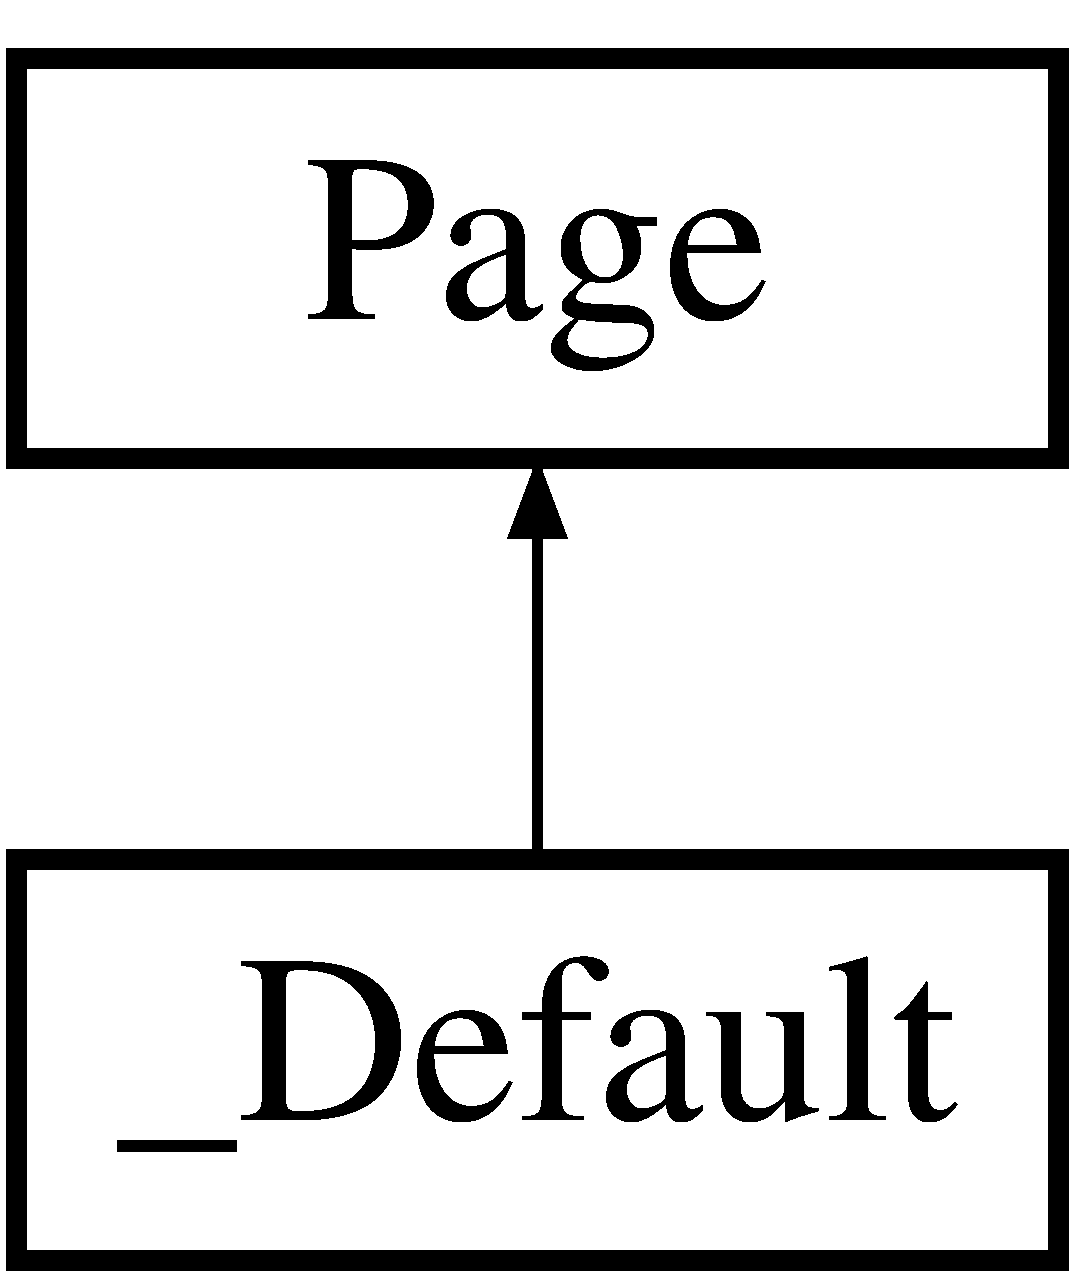
\includegraphics[height=2.000000cm]{class___default}
\end{center}
\end{figure}
\subsection*{Protected Member Functions}
\begin{DoxyCompactItemize}
\item 
\hypertarget{class___default_adacf7c92cb8d02f22ce02f0ceed897c1}{void {\bfseries Page\+\_\+\+Load} (object sender, Event\+Args e)}\label{class___default_adacf7c92cb8d02f22ce02f0ceed897c1}

\end{DoxyCompactItemize}


The documentation for this class was generated from the following file\+:\begin{DoxyCompactItemize}
\item 
H\+D3web/Default.\+aspx.\+cs\end{DoxyCompactItemize}

\hypertarget{class_devices}{\section{Devices Class Reference}
\label{class_devices}\index{Devices@{Devices}}
}
Inheritance diagram for Devices\+:\begin{figure}[H]
\begin{center}
\leavevmode
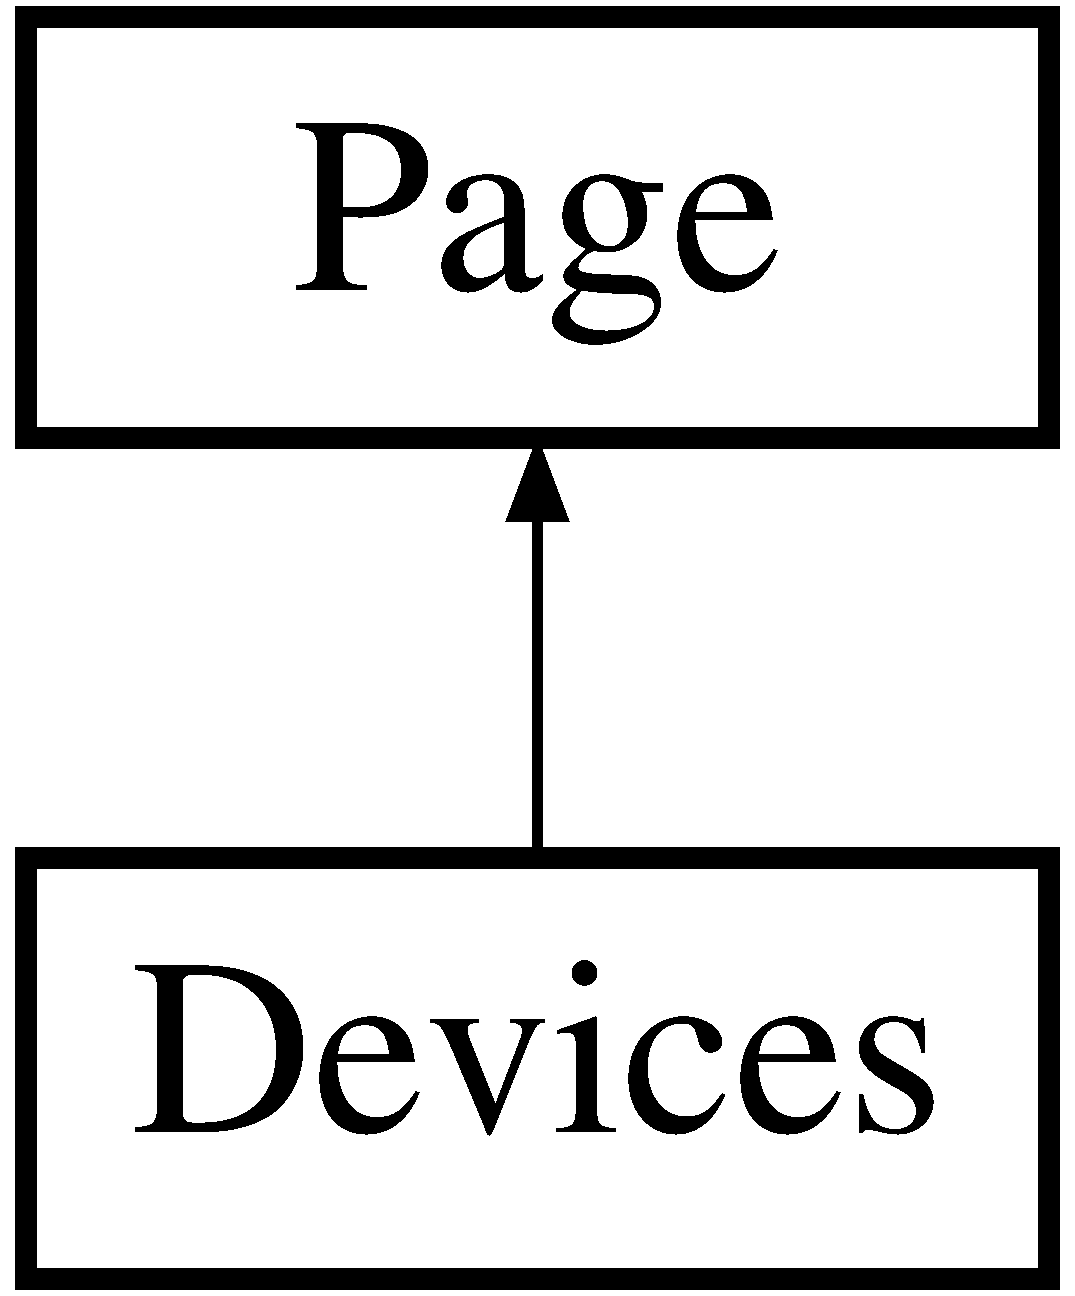
\includegraphics[height=2.000000cm]{class_devices}
\end{center}
\end{figure}
\subsection*{Protected Member Functions}
\begin{DoxyCompactItemize}
\item 
\hypertarget{class_devices_ab5e385bc09f2e7299cd68d6b518fc0c1}{void {\bfseries Page\+\_\+\+Load} (object sender, Event\+Args e)}\label{class_devices_ab5e385bc09f2e7299cd68d6b518fc0c1}

\end{DoxyCompactItemize}


The documentation for this class was generated from the following file\+:\begin{DoxyCompactItemize}
\item 
H\+D3web/Devices.\+aspx.\+cs\end{DoxyCompactItemize}

\hypertarget{class_h_d3_1_1_h_d3}{\section{H\+D3.\+H\+D3 Class Reference}
\label{class_h_d3_1_1_h_d3}\index{H\+D3.\+H\+D3@{H\+D3.\+H\+D3}}
}


Main class for all handset detection A\+P\+I calls  


\subsection*{Public Member Functions}
\begin{DoxyCompactItemize}
\item 
\hypertarget{class_h_d3_1_1_h_d3_a08cdeab81f9bddbfb126a7321ea2fd8c}{string {\bfseries get\+Raw\+Reply} ()}\label{class_h_d3_1_1_h_d3_a08cdeab81f9bddbfb126a7321ea2fd8c}

\item 
\hypertarget{class_h_d3_1_1_h_d3_ad79fcc6a7b1e5d38abc7219af87b3a2f}{dynamic {\bfseries get\+Reply} ()}\label{class_h_d3_1_1_h_d3_ad79fcc6a7b1e5d38abc7219af87b3a2f}

\item 
\hypertarget{class_h_d3_1_1_h_d3_a3dc243815bb91775b05d6fb148959983}{string {\bfseries get\+Error} ()}\label{class_h_d3_1_1_h_d3_a3dc243815bb91775b05d6fb148959983}

\item 
\hyperlink{class_h_d3_1_1_h_d3_a0a238bb9c0e43132312e5c863292c577}{H\+D3} (Http\+Request request)
\begin{DoxyCompactList}\small\item\em Initializes the necessary information for a lookup from request object Accepts Object inializers \end{DoxyCompactList}\item 
void \hyperlink{class_h_d3_1_1_h_d3_a658104a63e4bac0a909cdcfed8c2d49b}{set\+Detect\+Var} (string key, string val)
\begin{DoxyCompactList}\small\item\em Sets additional http headers for detection request, will override default headers.\end{DoxyCompactList}\item 
\hypertarget{class_h_d3_1_1_h_d3_a92e1a5bec8573497497bb7e4082a6b5c}{void {\bfseries reset\+Log} ()}\label{class_h_d3_1_1_h_d3_a92e1a5bec8573497497bb7e4082a6b5c}

\item 
\hypertarget{class_h_d3_1_1_h_d3_a2436e33681884291c6ad1b2ee112e17b}{string {\bfseries get\+Log} ()}\label{class_h_d3_1_1_h_d3_a2436e33681884291c6ad1b2ee112e17b}

\item 
\hypertarget{class_h_d3_1_1_h_d3_a0431d69035a8245a195f9060d5525790}{void {\bfseries clean\+Up} ()}\label{class_h_d3_1_1_h_d3_a0431d69035a8245a195f9060d5525790}

\item 
bool \hyperlink{class_h_d3_1_1_h_d3_aa2f63450321e2f47b2cb3baf8ff1a5e8}{device\+Vendors} ()
\begin{DoxyCompactList}\small\item\em Fetches all supported Vendors available at handsetdetection.\+com\end{DoxyCompactList}\item 
bool \hyperlink{class_h_d3_1_1_h_d3_a5af669048eb1d372a703dd53b242fe2f}{device\+Models} (string vendor)
\begin{DoxyCompactList}\small\item\em Fetches all available phone models in handsetdetection.\+com database. If a vendor is specified then only models for that vendor are returned. Call get\+Model() to get access to the returned list. \end{DoxyCompactList}\item 
bool \hyperlink{class_h_d3_1_1_h_d3_aaba6d717a4579ca6fa7c5727e5d92333}{device\+View} (string vendor, string model)
\begin{DoxyCompactList}\small\item\em Provides information on a handset given the vendor and model. \end{DoxyCompactList}\item 
bool \hyperlink{class_h_d3_1_1_h_d3_a9640edbaf4dd41cd1c8bec9fa86f53a6}{device\+What\+Has} (string key, string value)
\begin{DoxyCompactList}\small\item\em Provides information on a handset given the key and value. \end{DoxyCompactList}\item 
\hypertarget{class_h_d3_1_1_h_d3_a094f2de65aed6b70560ae08c8fabfb2b}{bool {\bfseries site\+Detect} (string options=\char`\"{}hd\+\_\+specs\char`\"{})}\label{class_h_d3_1_1_h_d3_a094f2de65aed6b70560ae08c8fabfb2b}

\item 
\hypertarget{class_h_d3_1_1_h_d3_ad40ca41ce8ab43e23d9fec5d69eb59b5}{bool {\bfseries site\+Fetch\+All} ()}\label{class_h_d3_1_1_h_d3_ad40ca41ce8ab43e23d9fec5d69eb59b5}

\item 
\hypertarget{class_h_d3_1_1_h_d3_ab7987ac1e6295533e55dcd5d300ae9cc}{bool {\bfseries site\+Fetch\+Trees} ()}\label{class_h_d3_1_1_h_d3_ab7987ac1e6295533e55dcd5d300ae9cc}

\item 
\hypertarget{class_h_d3_1_1_h_d3_ae8d86be9f088829ebe42214cfb26672e}{bool {\bfseries site\+Fetch\+Specs} ()}\label{class_h_d3_1_1_h_d3_ae8d86be9f088829ebe42214cfb26672e}

\item 
\hypertarget{class_h_d3_1_1_h_d3_a08cdeab81f9bddbfb126a7321ea2fd8c}{string {\bfseries get\+Raw\+Reply} ()}\label{class_h_d3_1_1_h_d3_a08cdeab81f9bddbfb126a7321ea2fd8c}

\item 
\hypertarget{class_h_d3_1_1_h_d3_ad79fcc6a7b1e5d38abc7219af87b3a2f}{dynamic {\bfseries get\+Reply} ()}\label{class_h_d3_1_1_h_d3_ad79fcc6a7b1e5d38abc7219af87b3a2f}

\item 
\hypertarget{class_h_d3_1_1_h_d3_a3dc243815bb91775b05d6fb148959983}{string {\bfseries get\+Error} ()}\label{class_h_d3_1_1_h_d3_a3dc243815bb91775b05d6fb148959983}

\item 
\hyperlink{class_h_d3_1_1_h_d3_a0a238bb9c0e43132312e5c863292c577}{H\+D3} (Http\+Request request)
\begin{DoxyCompactList}\small\item\em Initializes the necessary information for a lookup from request object Accepts Object inializers \end{DoxyCompactList}\item 
\hyperlink{class_h_d3_1_1_h_d3_a6f369b558b21414a20af987df0007a75}{H\+D3} ()
\begin{DoxyCompactList}\small\item\em No argument default constructor \end{DoxyCompactList}\item 
void \hyperlink{class_h_d3_1_1_h_d3_a658104a63e4bac0a909cdcfed8c2d49b}{set\+Detect\+Var} (string key, string val)
\begin{DoxyCompactList}\small\item\em Sets additional http headers for detection request, will override default headers.\end{DoxyCompactList}\item 
\hypertarget{class_h_d3_1_1_h_d3_a92e1a5bec8573497497bb7e4082a6b5c}{void {\bfseries reset\+Log} ()}\label{class_h_d3_1_1_h_d3_a92e1a5bec8573497497bb7e4082a6b5c}

\item 
\hypertarget{class_h_d3_1_1_h_d3_a2436e33681884291c6ad1b2ee112e17b}{string {\bfseries get\+Log} ()}\label{class_h_d3_1_1_h_d3_a2436e33681884291c6ad1b2ee112e17b}

\item 
\hypertarget{class_h_d3_1_1_h_d3_a0431d69035a8245a195f9060d5525790}{void {\bfseries clean\+Up} ()}\label{class_h_d3_1_1_h_d3_a0431d69035a8245a195f9060d5525790}

\item 
bool \hyperlink{class_h_d3_1_1_h_d3_aa2f63450321e2f47b2cb3baf8ff1a5e8}{device\+Vendors} ()
\begin{DoxyCompactList}\small\item\em Fetches all supported Vendors available at handsetdetection.\+com\end{DoxyCompactList}\item 
bool \hyperlink{class_h_d3_1_1_h_d3_a5af669048eb1d372a703dd53b242fe2f}{device\+Models} (string vendor)
\begin{DoxyCompactList}\small\item\em Fetches all available phone models in handsetdetection.\+com database. If a vendor is specified then only models for that vendor are returned. Call get\+Model() to get access to the returned list. \end{DoxyCompactList}\item 
bool \hyperlink{class_h_d3_1_1_h_d3_aaba6d717a4579ca6fa7c5727e5d92333}{device\+View} (string vendor, string model)
\begin{DoxyCompactList}\small\item\em Provides information on a handset given the vendor and model. \end{DoxyCompactList}\item 
bool \hyperlink{class_h_d3_1_1_h_d3_a9640edbaf4dd41cd1c8bec9fa86f53a6}{device\+What\+Has} (string key, string value)
\begin{DoxyCompactList}\small\item\em Provides information on a handset given the key and value. \end{DoxyCompactList}\item 
\hypertarget{class_h_d3_1_1_h_d3_a094f2de65aed6b70560ae08c8fabfb2b}{bool {\bfseries site\+Detect} (string options=\char`\"{}hd\+\_\+specs\char`\"{})}\label{class_h_d3_1_1_h_d3_a094f2de65aed6b70560ae08c8fabfb2b}

\item 
bool \hyperlink{class_h_d3_1_1_h_d3_ad40ca41ce8ab43e23d9fec5d69eb59b5}{site\+Fetch\+All} ()
\item 
bool \hyperlink{class_h_d3_1_1_h_d3_ab7987ac1e6295533e55dcd5d300ae9cc}{site\+Fetch\+Trees} ()
\item 
bool \hyperlink{class_h_d3_1_1_h_d3_ae8d86be9f088829ebe42214cfb26672e}{site\+Fetch\+Specs} ()
\end{DoxyCompactItemize}
\subsection*{Public Attributes}
\begin{DoxyCompactItemize}
\item 
\hypertarget{class_h_d3_1_1_h_d3_af413d17666d552b40589ad290802f868}{string {\bfseries log} = \char`\"{}\char`\"{}}\label{class_h_d3_1_1_h_d3_af413d17666d552b40589ad290802f868}

\end{DoxyCompactItemize}
\subsection*{Properties}
\begin{DoxyCompactItemize}
\item 
\hypertarget{class_h_d3_1_1_h_d3_a52ca1bb216ac5a05d0f97780b5b16dee}{int {\bfseries Read\+Timeout}\hspace{0.3cm}{\ttfamily  \mbox{[}get, set\mbox{]}}}\label{class_h_d3_1_1_h_d3_a52ca1bb216ac5a05d0f97780b5b16dee}

\item 
\hypertarget{class_h_d3_1_1_h_d3_a9fbf3afb5c9b20dbd781c74864fbed59}{int {\bfseries Connect\+Timeout}\hspace{0.3cm}{\ttfamily  \mbox{[}get, set\mbox{]}}}\label{class_h_d3_1_1_h_d3_a9fbf3afb5c9b20dbd781c74864fbed59}

\item 
\hypertarget{class_h_d3_1_1_h_d3_af24410685eb95084649ac58b24e5349e}{string {\bfseries Username}\hspace{0.3cm}{\ttfamily  \mbox{[}get, set\mbox{]}}}\label{class_h_d3_1_1_h_d3_af24410685eb95084649ac58b24e5349e}

\item 
\hypertarget{class_h_d3_1_1_h_d3_ac95f6be2551f612f59bad083abacfb42}{string {\bfseries Secret}\hspace{0.3cm}{\ttfamily  \mbox{[}get, set\mbox{]}}}\label{class_h_d3_1_1_h_d3_ac95f6be2551f612f59bad083abacfb42}

\item 
\hypertarget{class_h_d3_1_1_h_d3_a2aaf415e233764b3da83eacaeab7d62d}{string {\bfseries Site\+Id}\hspace{0.3cm}{\ttfamily  \mbox{[}get, set\mbox{]}}}\label{class_h_d3_1_1_h_d3_a2aaf415e233764b3da83eacaeab7d62d}

\item 
\hypertarget{class_h_d3_1_1_h_d3_a0d7be479af393a7f9e17d329f123db41}{bool {\bfseries Use\+Local}\hspace{0.3cm}{\ttfamily  \mbox{[}get, set\mbox{]}}}\label{class_h_d3_1_1_h_d3_a0d7be479af393a7f9e17d329f123db41}

\item 
\hypertarget{class_h_d3_1_1_h_d3_a812cd4c1d783d795ea5eb013cd2e9e9b}{bool {\bfseries Use\+Proxy}\hspace{0.3cm}{\ttfamily  \mbox{[}get, set\mbox{]}}}\label{class_h_d3_1_1_h_d3_a812cd4c1d783d795ea5eb013cd2e9e9b}

\item 
\hypertarget{class_h_d3_1_1_h_d3_a964cd4701dc83befef4e9c0fd8e21462}{string {\bfseries Proxy\+Server}\hspace{0.3cm}{\ttfamily  \mbox{[}get, set\mbox{]}}}\label{class_h_d3_1_1_h_d3_a964cd4701dc83befef4e9c0fd8e21462}

\item 
\hypertarget{class_h_d3_1_1_h_d3_af92cba5e3de6cca12335a77423ba3413}{string {\bfseries Proxy\+Port}\hspace{0.3cm}{\ttfamily  \mbox{[}get, set\mbox{]}}}\label{class_h_d3_1_1_h_d3_af92cba5e3de6cca12335a77423ba3413}

\item 
\hypertarget{class_h_d3_1_1_h_d3_a4ccc6ceb0f1535917177d94ca8bb8def}{string {\bfseries Proxy\+Pass}\hspace{0.3cm}{\ttfamily  \mbox{[}get, set\mbox{]}}}\label{class_h_d3_1_1_h_d3_a4ccc6ceb0f1535917177d94ca8bb8def}

\item 
\hypertarget{class_h_d3_1_1_h_d3_a552e44bcefd4244b7279abf1dc2c10fb}{string {\bfseries Proxy\+User}\hspace{0.3cm}{\ttfamily  \mbox{[}get, set\mbox{]}}}\label{class_h_d3_1_1_h_d3_a552e44bcefd4244b7279abf1dc2c10fb}

\item 
\hypertarget{class_h_d3_1_1_h_d3_a35d1f45be522060d497b7ee727dd1e36}{string {\bfseries Match\+Filter}\hspace{0.3cm}{\ttfamily  \mbox{[}get, set\mbox{]}}}\label{class_h_d3_1_1_h_d3_a35d1f45be522060d497b7ee727dd1e36}

\item 
\hypertarget{class_h_d3_1_1_h_d3_a6af54b9273944f22dfa1d04b0441f73f}{string {\bfseries Non\+Mobile}\hspace{0.3cm}{\ttfamily  \mbox{[}get, set\mbox{]}}}\label{class_h_d3_1_1_h_d3_a6af54b9273944f22dfa1d04b0441f73f}

\item 
\hypertarget{class_h_d3_1_1_h_d3_ac6d923a19fa138b6eab2882121106640}{string {\bfseries Api\+Server}\hspace{0.3cm}{\ttfamily  \mbox{[}get, set\mbox{]}}}\label{class_h_d3_1_1_h_d3_ac6d923a19fa138b6eab2882121106640}

\item 
\hypertarget{class_h_d3_1_1_h_d3_a931745a4ed8826fffcf43c010ee80531}{string {\bfseries Log\+Server}\hspace{0.3cm}{\ttfamily  \mbox{[}get, set\mbox{]}}}\label{class_h_d3_1_1_h_d3_a931745a4ed8826fffcf43c010ee80531}

\end{DoxyCompactItemize}


\subsection{Detailed Description}
Main class for all handset detection A\+P\+I calls 



\subsection{Constructor \& Destructor Documentation}
\hypertarget{class_h_d3_1_1_h_d3_a0a238bb9c0e43132312e5c863292c577}{\index{H\+D3\+::\+H\+D3@{H\+D3\+::\+H\+D3}!H\+D3@{H\+D3}}
\index{H\+D3@{H\+D3}!H\+D3\+::\+H\+D3@{H\+D3\+::\+H\+D3}}
\subsubsection[{H\+D3}]{\setlength{\rightskip}{0pt plus 5cm}H\+D3.\+H\+D3.\+H\+D3 (
\begin{DoxyParamCaption}
\item[{Http\+Request}]{request}
\end{DoxyParamCaption}
)\hspace{0.3cm}{\ttfamily [inline]}}}\label{class_h_d3_1_1_h_d3_a0a238bb9c0e43132312e5c863292c577}


Initializes the necessary information for a lookup from request object Accepts Object inializers 


\begin{DoxyParams}{Parameters}
{\em request} & Http\+Request object from page\\
\hline
\end{DoxyParams}
\hypertarget{class_h_d3_1_1_h_d3_a0a238bb9c0e43132312e5c863292c577}{\index{H\+D3\+::\+H\+D3@{H\+D3\+::\+H\+D3}!H\+D3@{H\+D3}}
\index{H\+D3@{H\+D3}!H\+D3\+::\+H\+D3@{H\+D3\+::\+H\+D3}}
\subsubsection[{H\+D3}]{\setlength{\rightskip}{0pt plus 5cm}H\+D3.\+H\+D3.\+H\+D3 (
\begin{DoxyParamCaption}
\item[{Http\+Request}]{request}
\end{DoxyParamCaption}
)\hspace{0.3cm}{\ttfamily [inline]}}}\label{class_h_d3_1_1_h_d3_a0a238bb9c0e43132312e5c863292c577}


Initializes the necessary information for a lookup from request object Accepts Object inializers 


\begin{DoxyParams}{Parameters}
{\em request} & Http\+Request object from page\\
\hline
\end{DoxyParams}
\hypertarget{class_h_d3_1_1_h_d3_a6f369b558b21414a20af987df0007a75}{\index{H\+D3\+::\+H\+D3@{H\+D3\+::\+H\+D3}!H\+D3@{H\+D3}}
\index{H\+D3@{H\+D3}!H\+D3\+::\+H\+D3@{H\+D3\+::\+H\+D3}}
\subsubsection[{H\+D3}]{\setlength{\rightskip}{0pt plus 5cm}H\+D3.\+H\+D3.\+H\+D3 (
\begin{DoxyParamCaption}
{}
\end{DoxyParamCaption}
)\hspace{0.3cm}{\ttfamily [inline]}}}\label{class_h_d3_1_1_h_d3_a6f369b558b21414a20af987df0007a75}


No argument default constructor 



\subsection{Member Function Documentation}
\hypertarget{class_h_d3_1_1_h_d3_a5af669048eb1d372a703dd53b242fe2f}{\index{H\+D3\+::\+H\+D3@{H\+D3\+::\+H\+D3}!device\+Models@{device\+Models}}
\index{device\+Models@{device\+Models}!H\+D3\+::\+H\+D3@{H\+D3\+::\+H\+D3}}
\subsubsection[{device\+Models}]{\setlength{\rightskip}{0pt plus 5cm}bool H\+D3.\+H\+D3.\+device\+Models (
\begin{DoxyParamCaption}
\item[{string}]{vendor}
\end{DoxyParamCaption}
)\hspace{0.3cm}{\ttfamily [inline]}}}\label{class_h_d3_1_1_h_d3_a5af669048eb1d372a703dd53b242fe2f}


Fetches all available phone models in handsetdetection.\+com database. If a vendor is specified then only models for that vendor are returned. Call get\+Model() to get access to the returned list. 


\begin{DoxyParams}{Parameters}
{\em vendor} & all or a valid vendor name\\
\hline
\end{DoxyParams}
\begin{DoxyReturn}{Returns}
true if successful, false otherwise
\end{DoxyReturn}
\hypertarget{class_h_d3_1_1_h_d3_a5af669048eb1d372a703dd53b242fe2f}{\index{H\+D3\+::\+H\+D3@{H\+D3\+::\+H\+D3}!device\+Models@{device\+Models}}
\index{device\+Models@{device\+Models}!H\+D3\+::\+H\+D3@{H\+D3\+::\+H\+D3}}
\subsubsection[{device\+Models}]{\setlength{\rightskip}{0pt plus 5cm}bool H\+D3.\+H\+D3.\+device\+Models (
\begin{DoxyParamCaption}
\item[{string}]{vendor}
\end{DoxyParamCaption}
)\hspace{0.3cm}{\ttfamily [inline]}}}\label{class_h_d3_1_1_h_d3_a5af669048eb1d372a703dd53b242fe2f}


Fetches all available phone models in handsetdetection.\+com database. If a vendor is specified then only models for that vendor are returned. Call get\+Model() to get access to the returned list. 


\begin{DoxyParams}{Parameters}
{\em vendor} & all or a valid vendor name\\
\hline
\end{DoxyParams}
\begin{DoxyReturn}{Returns}
true if successful, false otherwise
\end{DoxyReturn}
\hypertarget{class_h_d3_1_1_h_d3_aa2f63450321e2f47b2cb3baf8ff1a5e8}{\index{H\+D3\+::\+H\+D3@{H\+D3\+::\+H\+D3}!device\+Vendors@{device\+Vendors}}
\index{device\+Vendors@{device\+Vendors}!H\+D3\+::\+H\+D3@{H\+D3\+::\+H\+D3}}
\subsubsection[{device\+Vendors}]{\setlength{\rightskip}{0pt plus 5cm}bool H\+D3.\+H\+D3.\+device\+Vendors (
\begin{DoxyParamCaption}
{}
\end{DoxyParamCaption}
)\hspace{0.3cm}{\ttfamily [inline]}}}\label{class_h_d3_1_1_h_d3_aa2f63450321e2f47b2cb3baf8ff1a5e8}


Fetches all supported Vendors available at handsetdetection.\+com

\begin{DoxyReturn}{Returns}
true if successful, false otherwise
\end{DoxyReturn}
\hypertarget{class_h_d3_1_1_h_d3_aa2f63450321e2f47b2cb3baf8ff1a5e8}{\index{H\+D3\+::\+H\+D3@{H\+D3\+::\+H\+D3}!device\+Vendors@{device\+Vendors}}
\index{device\+Vendors@{device\+Vendors}!H\+D3\+::\+H\+D3@{H\+D3\+::\+H\+D3}}
\subsubsection[{device\+Vendors}]{\setlength{\rightskip}{0pt plus 5cm}bool H\+D3.\+H\+D3.\+device\+Vendors (
\begin{DoxyParamCaption}
{}
\end{DoxyParamCaption}
)\hspace{0.3cm}{\ttfamily [inline]}}}\label{class_h_d3_1_1_h_d3_aa2f63450321e2f47b2cb3baf8ff1a5e8}


Fetches all supported Vendors available at handsetdetection.\+com

\begin{DoxyReturn}{Returns}
true if successful, false otherwise
\end{DoxyReturn}
\hypertarget{class_h_d3_1_1_h_d3_aaba6d717a4579ca6fa7c5727e5d92333}{\index{H\+D3\+::\+H\+D3@{H\+D3\+::\+H\+D3}!device\+View@{device\+View}}
\index{device\+View@{device\+View}!H\+D3\+::\+H\+D3@{H\+D3\+::\+H\+D3}}
\subsubsection[{device\+View}]{\setlength{\rightskip}{0pt plus 5cm}bool H\+D3.\+H\+D3.\+device\+View (
\begin{DoxyParamCaption}
\item[{string}]{vendor, }
\item[{string}]{model}
\end{DoxyParamCaption}
)\hspace{0.3cm}{\ttfamily [inline]}}}\label{class_h_d3_1_1_h_d3_aaba6d717a4579ca6fa7c5727e5d92333}


Provides information on a handset given the vendor and model. 


\begin{DoxyParams}{Parameters}
{\em vendor} & vendor\\
\hline
{\em model} & model\\
\hline
\end{DoxyParams}
\begin{DoxyReturn}{Returns}
true if successful, false otherwise
\end{DoxyReturn}
\hypertarget{class_h_d3_1_1_h_d3_aaba6d717a4579ca6fa7c5727e5d92333}{\index{H\+D3\+::\+H\+D3@{H\+D3\+::\+H\+D3}!device\+View@{device\+View}}
\index{device\+View@{device\+View}!H\+D3\+::\+H\+D3@{H\+D3\+::\+H\+D3}}
\subsubsection[{device\+View}]{\setlength{\rightskip}{0pt plus 5cm}bool H\+D3.\+H\+D3.\+device\+View (
\begin{DoxyParamCaption}
\item[{string}]{vendor, }
\item[{string}]{model}
\end{DoxyParamCaption}
)\hspace{0.3cm}{\ttfamily [inline]}}}\label{class_h_d3_1_1_h_d3_aaba6d717a4579ca6fa7c5727e5d92333}


Provides information on a handset given the vendor and model. 


\begin{DoxyParams}{Parameters}
{\em vendor} & vendor\\
\hline
{\em model} & model\\
\hline
\end{DoxyParams}
\begin{DoxyReturn}{Returns}
true if successful, false otherwise
\end{DoxyReturn}
\hypertarget{class_h_d3_1_1_h_d3_a9640edbaf4dd41cd1c8bec9fa86f53a6}{\index{H\+D3\+::\+H\+D3@{H\+D3\+::\+H\+D3}!device\+What\+Has@{device\+What\+Has}}
\index{device\+What\+Has@{device\+What\+Has}!H\+D3\+::\+H\+D3@{H\+D3\+::\+H\+D3}}
\subsubsection[{device\+What\+Has}]{\setlength{\rightskip}{0pt plus 5cm}bool H\+D3.\+H\+D3.\+device\+What\+Has (
\begin{DoxyParamCaption}
\item[{string}]{key, }
\item[{string}]{value}
\end{DoxyParamCaption}
)\hspace{0.3cm}{\ttfamily [inline]}}}\label{class_h_d3_1_1_h_d3_a9640edbaf4dd41cd1c8bec9fa86f53a6}


Provides information on a handset given the key and value. 


\begin{DoxyParams}{Parameters}
{\em key} & key\\
\hline
{\em value} & value\\
\hline
\end{DoxyParams}
\begin{DoxyReturn}{Returns}

\end{DoxyReturn}
\hypertarget{class_h_d3_1_1_h_d3_a9640edbaf4dd41cd1c8bec9fa86f53a6}{\index{H\+D3\+::\+H\+D3@{H\+D3\+::\+H\+D3}!device\+What\+Has@{device\+What\+Has}}
\index{device\+What\+Has@{device\+What\+Has}!H\+D3\+::\+H\+D3@{H\+D3\+::\+H\+D3}}
\subsubsection[{device\+What\+Has}]{\setlength{\rightskip}{0pt plus 5cm}bool H\+D3.\+H\+D3.\+device\+What\+Has (
\begin{DoxyParamCaption}
\item[{string}]{key, }
\item[{string}]{value}
\end{DoxyParamCaption}
)\hspace{0.3cm}{\ttfamily [inline]}}}\label{class_h_d3_1_1_h_d3_a9640edbaf4dd41cd1c8bec9fa86f53a6}


Provides information on a handset given the key and value. 


\begin{DoxyParams}{Parameters}
{\em key} & key\\
\hline
{\em value} & value\\
\hline
\end{DoxyParams}
\begin{DoxyReturn}{Returns}

\end{DoxyReturn}
\hypertarget{class_h_d3_1_1_h_d3_a658104a63e4bac0a909cdcfed8c2d49b}{\index{H\+D3\+::\+H\+D3@{H\+D3\+::\+H\+D3}!set\+Detect\+Var@{set\+Detect\+Var}}
\index{set\+Detect\+Var@{set\+Detect\+Var}!H\+D3\+::\+H\+D3@{H\+D3\+::\+H\+D3}}
\subsubsection[{set\+Detect\+Var}]{\setlength{\rightskip}{0pt plus 5cm}void H\+D3.\+H\+D3.\+set\+Detect\+Var (
\begin{DoxyParamCaption}
\item[{string}]{key, }
\item[{string}]{val}
\end{DoxyParamCaption}
)\hspace{0.3cm}{\ttfamily [inline]}}}\label{class_h_d3_1_1_h_d3_a658104a63e4bac0a909cdcfed8c2d49b}


Sets additional http headers for detection request, will override default headers.


\begin{DoxyParams}{Parameters}
{\em key} & \\
\hline
{\em val} & \\
\hline
\end{DoxyParams}
\hypertarget{class_h_d3_1_1_h_d3_a658104a63e4bac0a909cdcfed8c2d49b}{\index{H\+D3\+::\+H\+D3@{H\+D3\+::\+H\+D3}!set\+Detect\+Var@{set\+Detect\+Var}}
\index{set\+Detect\+Var@{set\+Detect\+Var}!H\+D3\+::\+H\+D3@{H\+D3\+::\+H\+D3}}
\subsubsection[{set\+Detect\+Var}]{\setlength{\rightskip}{0pt plus 5cm}void H\+D3.\+H\+D3.\+set\+Detect\+Var (
\begin{DoxyParamCaption}
\item[{string}]{key, }
\item[{string}]{val}
\end{DoxyParamCaption}
)\hspace{0.3cm}{\ttfamily [inline]}}}\label{class_h_d3_1_1_h_d3_a658104a63e4bac0a909cdcfed8c2d49b}


Sets additional http headers for detection request, will override default headers.


\begin{DoxyParams}{Parameters}
{\em key} & \\
\hline
{\em val} & \\
\hline
\end{DoxyParams}
\hypertarget{class_h_d3_1_1_h_d3_ad40ca41ce8ab43e23d9fec5d69eb59b5}{\index{H\+D3\+::\+H\+D3@{H\+D3\+::\+H\+D3}!site\+Fetch\+All@{site\+Fetch\+All}}
\index{site\+Fetch\+All@{site\+Fetch\+All}!H\+D3\+::\+H\+D3@{H\+D3\+::\+H\+D3}}
\subsubsection[{site\+Fetch\+All}]{\setlength{\rightskip}{0pt plus 5cm}bool H\+D3.\+H\+D3.\+site\+Fetch\+All (
\begin{DoxyParamCaption}
{}
\end{DoxyParamCaption}
)\hspace{0.3cm}{\ttfamily [inline]}}}\label{class_h_d3_1_1_h_d3_ad40ca41ce8ab43e23d9fec5d69eb59b5}




\begin{DoxyReturn}{Returns}

\end{DoxyReturn}
\hypertarget{class_h_d3_1_1_h_d3_ae8d86be9f088829ebe42214cfb26672e}{\index{H\+D3\+::\+H\+D3@{H\+D3\+::\+H\+D3}!site\+Fetch\+Specs@{site\+Fetch\+Specs}}
\index{site\+Fetch\+Specs@{site\+Fetch\+Specs}!H\+D3\+::\+H\+D3@{H\+D3\+::\+H\+D3}}
\subsubsection[{site\+Fetch\+Specs}]{\setlength{\rightskip}{0pt plus 5cm}bool H\+D3.\+H\+D3.\+site\+Fetch\+Specs (
\begin{DoxyParamCaption}
{}
\end{DoxyParamCaption}
)\hspace{0.3cm}{\ttfamily [inline]}}}\label{class_h_d3_1_1_h_d3_ae8d86be9f088829ebe42214cfb26672e}




\begin{DoxyReturn}{Returns}

\end{DoxyReturn}
\hypertarget{class_h_d3_1_1_h_d3_ab7987ac1e6295533e55dcd5d300ae9cc}{\index{H\+D3\+::\+H\+D3@{H\+D3\+::\+H\+D3}!site\+Fetch\+Trees@{site\+Fetch\+Trees}}
\index{site\+Fetch\+Trees@{site\+Fetch\+Trees}!H\+D3\+::\+H\+D3@{H\+D3\+::\+H\+D3}}
\subsubsection[{site\+Fetch\+Trees}]{\setlength{\rightskip}{0pt plus 5cm}bool H\+D3.\+H\+D3.\+site\+Fetch\+Trees (
\begin{DoxyParamCaption}
{}
\end{DoxyParamCaption}
)\hspace{0.3cm}{\ttfamily [inline]}}}\label{class_h_d3_1_1_h_d3_ab7987ac1e6295533e55dcd5d300ae9cc}




\begin{DoxyReturn}{Returns}

\end{DoxyReturn}


The documentation for this class was generated from the following files\+:\begin{DoxyCompactItemize}
\item 
C\+:/\+Users/\+Bobcat/\+Desktop/\+Handset\+Detection/dotnet40-\/apikit/\+H\+D3lib/H\+D3-\/mine.\+cs\item 
C\+:/\+Users/\+Bobcat/\+Desktop/\+Handset\+Detection/dotnet40-\/apikit/\+H\+D3lib/H\+D3.\+cs\end{DoxyCompactItemize}

\hypertarget{class_h_d3_1_1_h_d3_cache}{\section{H\+D3.\+H\+D3\+Cache Class Reference}
\label{class_h_d3_1_1_h_d3_cache}\index{H\+D3.\+H\+D3\+Cache@{H\+D3.\+H\+D3\+Cache}}
}
\subsection*{Public Member Functions}
\begin{DoxyCompactItemize}
\item 
void \hyperlink{class_h_d3_1_1_h_d3_cache_a216ecd26c7f8c28f7b9283470ab5f944}{write} (string key, dynamic value)
\begin{DoxyCompactList}\small\item\em Write new object to dictionary \end{DoxyCompactList}\item 
Dictionary$<$ string, dynamic $>$ \hyperlink{class_h_d3_1_1_h_d3_cache_aee9c64f3dd4ee57f8bc4b552b984761f}{read} (string key)
\begin{DoxyCompactList}\small\item\em Read object from dictionary \end{DoxyCompactList}\end{DoxyCompactItemize}


\subsection{Detailed Description}
The \hyperlink{class_h_d3_1_1_h_d3_cache}{H\+D3\+Cache} class /\+Summary$>$ 

\subsection{Member Function Documentation}
\hypertarget{class_h_d3_1_1_h_d3_cache_aee9c64f3dd4ee57f8bc4b552b984761f}{\index{H\+D3\+::\+H\+D3\+Cache@{H\+D3\+::\+H\+D3\+Cache}!read@{read}}
\index{read@{read}!H\+D3\+::\+H\+D3\+Cache@{H\+D3\+::\+H\+D3\+Cache}}
\subsubsection[{read}]{\setlength{\rightskip}{0pt plus 5cm}Dictionary$<$string, dynamic$>$ H\+D3.\+H\+D3\+Cache.\+read (
\begin{DoxyParamCaption}
\item[{string}]{key}
\end{DoxyParamCaption}
)\hspace{0.3cm}{\ttfamily [inline]}}}\label{class_h_d3_1_1_h_d3_cache_aee9c64f3dd4ee57f8bc4b552b984761f}


Read object from dictionary 


\begin{DoxyParams}{Parameters}
{\em key} & \\
\hline
\end{DoxyParams}
\begin{DoxyReturn}{Returns}

\end{DoxyReturn}
\hypertarget{class_h_d3_1_1_h_d3_cache_a216ecd26c7f8c28f7b9283470ab5f944}{\index{H\+D3\+::\+H\+D3\+Cache@{H\+D3\+::\+H\+D3\+Cache}!write@{write}}
\index{write@{write}!H\+D3\+::\+H\+D3\+Cache@{H\+D3\+::\+H\+D3\+Cache}}
\subsubsection[{write}]{\setlength{\rightskip}{0pt plus 5cm}void H\+D3.\+H\+D3\+Cache.\+write (
\begin{DoxyParamCaption}
\item[{string}]{key, }
\item[{dynamic}]{value}
\end{DoxyParamCaption}
)\hspace{0.3cm}{\ttfamily [inline]}}}\label{class_h_d3_1_1_h_d3_cache_a216ecd26c7f8c28f7b9283470ab5f944}


Write new object to dictionary 


\begin{DoxyParams}{Parameters}
{\em key} & \\
\hline
{\em value} & \\
\hline
\end{DoxyParams}


The documentation for this class was generated from the following file\+:\begin{DoxyCompactItemize}
\item 
H\+D3.\+cs\end{DoxyCompactItemize}

\hypertarget{class_h_d3_1_1_test_1_1_h_d3_test}{\section{H\+D3.\+Test.\+H\+D3\+Test Class Reference}
\label{class_h_d3_1_1_test_1_1_h_d3_test}\index{H\+D3.\+Test.\+H\+D3\+Test@{H\+D3.\+Test.\+H\+D3\+Test}}
}
\subsection*{Public Member Functions}
\begin{DoxyCompactItemize}
\item 
void \hyperlink{class_h_d3_1_1_test_1_1_h_d3_test_ae9e28970c4958a3e32fcb32f8138c450}{Initialize} ()
\begin{DoxyCompactList}\small\item\em initialize objects \end{DoxyCompactList}\item 
void \hyperlink{class_h_d3_1_1_test_1_1_h_d3_test_acd440d651771abea6c4f7bec066b8fc9}{Test\+\_\+\+Username\+Required} ()
\begin{DoxyCompactList}\small\item\em \hyperlink{namespace_h_d3_1_1_test}{Test} for runtime exception \end{DoxyCompactList}\item 
void \hyperlink{class_h_d3_1_1_test_1_1_h_d3_test_a6e43154f24d0068475a0dccdd27ed0b1}{Test\+\_\+\+Secret\+Required} ()
\begin{DoxyCompactList}\small\item\em \hyperlink{namespace_h_d3_1_1_test}{Test} for runtime exception \end{DoxyCompactList}\item 
void \hyperlink{class_h_d3_1_1_test_1_1_h_d3_test_a6164a00d42c805f748af17e88cde7f96}{Test\+\_\+\+Passed\+Config} ()
\begin{DoxyCompactList}\small\item\em \hyperlink{namespace_h_d3_1_1_test}{Test} for a config passed to the constructor \end{DoxyCompactList}\item 
void \hyperlink{class_h_d3_1_1_test_1_1_h_d3_test_a5c2635c61ef62aef235f1c3013b5118a}{Test\+\_\+\+Default\+File\+Config} ()
\begin{DoxyCompactList}\small\item\em \hyperlink{namespace_h_d3_1_1_test}{Test} for default config readon from config file \end{DoxyCompactList}\item 
void \hyperlink{class_h_d3_1_1_test_1_1_h_d3_test_ae0d5998f007f3d055bea00589a744668}{Test\+\_\+\+Default\+Setup} ()
\begin{DoxyCompactList}\small\item\em \hyperlink{namespace_h_d3_1_1_test}{Test} for default http headers read when a new object is instantiated \end{DoxyCompactList}\item 
void \hyperlink{class_h_d3_1_1_test_1_1_h_d3_test_a586e6f5874d7946b5294fb6ff3fa4acd}{Test\+\_\+\+Manual\+Setup} ()
\begin{DoxyCompactList}\small\item\em \hyperlink{namespace_h_d3_1_1_test}{Test} for manual setting of http headers \end{DoxyCompactList}\item 
void \hyperlink{class_h_d3_1_1_test_1_1_h_d3_test_a7f6749b2ad203c4cc782af151787d70a}{Test\+\_\+\+Invalid\+Credentials} ()
\begin{DoxyCompactList}\small\item\em \hyperlink{namespace_h_d3_1_1_test}{Test} for invalis A\+P\+I credentials \end{DoxyCompactList}\item 
void \hyperlink{class_h_d3_1_1_test_1_1_h_d3_test_a8c45dad93eac37046ff73898012d94e0}{Device\+Vendors} (bool local, bool proxy)
\begin{DoxyCompactList}\small\item\em The list is continually growing so ensure its a min length and common vendors are present \end{DoxyCompactList}\item 
void \hyperlink{class_h_d3_1_1_test_1_1_h_d3_test_a358f5267e8cf30c24931cbf3692af1ae}{Test\+\_\+\+Device\+Vendors\+Fail} ()
\begin{DoxyCompactList}\small\item\em The list is continually growing so ensure its a min length and common vendors are present \end{DoxyCompactList}\item 
void \hyperlink{class_h_d3_1_1_test_1_1_h_d3_test_a2adb09017cb44d368c271f12af27e3e2}{Device\+Models} (bool local, bool proxy)
\begin{DoxyCompactList}\small\item\em This list is also continually growing so ensure its a minimum length \end{DoxyCompactList}\item 
void \hyperlink{class_h_d3_1_1_test_1_1_h_d3_test_a495b9e3d48918da6aeb416b5d4291f7a}{Device\+View} (bool local, bool proxy)
\begin{DoxyCompactList}\small\item\em View detailed information about one device \end{DoxyCompactList}\item 
void \hyperlink{class_h_d3_1_1_test_1_1_h_d3_test_a60e604c7c80fe95810989db32be9a68c}{Device\+What\+Has} (bool local, bool proxy)
\begin{DoxyCompactList}\small\item\em Find which devices have a specific property \end{DoxyCompactList}\item 
void \hyperlink{class_h_d3_1_1_test_1_1_h_d3_test_a7574fbc39a251aa2d73b923c41612db5}{Site\+Detect} (bool local, bool proxy)
\begin{DoxyCompactList}\small\item\em Perform a battery of detection tests \end{DoxyCompactList}\item 
void \hyperlink{class_h_d3_1_1_test_1_1_h_d3_test_ac33dd7669508077165ee77c241904f6a}{Test\+\_\+\+Nokia\+Site\+Detect} ()
\begin{DoxyCompactList}\small\item\em \hyperlink{namespace_h_d3_1_1_test}{Test} device nokia browser detect \end{DoxyCompactList}\item 
void \hyperlink{class_h_d3_1_1_test_1_1_h_d3_test_abdbc11cf1956c40b5f0894f05654ec70}{Test\+\_\+\+Device\+Vendors\+Found} ()
\begin{DoxyCompactList}\small\item\em \hyperlink{namespace_h_d3_1_1_test}{Test} device vendors found \end{DoxyCompactList}\item 
void \hyperlink{class_h_d3_1_1_test_1_1_h_d3_test_a474e2044227b1931e1d29127b3e4e3be}{Test\+\_\+\+Device\+Vendors\+Not\+Found} ()
\begin{DoxyCompactList}\small\item\em \hyperlink{namespace_h_d3_1_1_test}{Test} devices vendors not found \end{DoxyCompactList}\item 
void \hyperlink{class_h_d3_1_1_test_1_1_h_d3_test_aa9cc42b177f48b4712f863e108c0a9f4}{Test\+\_\+\+Device\+Models\+Nokia\+Pass} ()
\begin{DoxyCompactList}\small\item\em \hyperlink{namespace_h_d3_1_1_test}{Test} device nokia models; true \end{DoxyCompactList}\item 
void \hyperlink{class_h_d3_1_1_test_1_1_h_d3_test_acb1b39078dc55c7d0f845bfd5fd05767}{Test\+\_\+\+Device\+Models\+Nokia\+Fail} ()
\begin{DoxyCompactList}\small\item\em \hyperlink{namespace_h_d3_1_1_test}{Test} device nokia models; false \end{DoxyCompactList}\item 
void \hyperlink{class_h_d3_1_1_test_1_1_h_d3_test_af83c75a963ca9c63386bd6056072e4f4}{Test\+\_\+\+Device\+View\+Nokia95} ()
\begin{DoxyCompactList}\small\item\em \hyperlink{namespace_h_d3_1_1_test}{Test} device view nokia n95 \end{DoxyCompactList}\item 
void \hyperlink{class_h_d3_1_1_test_1_1_h_d3_test_a0a6aec72c58863377b561115606a270b}{Test\+\_\+\+Device\+View\+Apple\+I\+Phone5s} ()
\begin{DoxyCompactList}\small\item\em \hyperlink{namespace_h_d3_1_1_test}{Test} device view apple iphone 5s \end{DoxyCompactList}\item 
void \hyperlink{class_h_d3_1_1_test_1_1_h_d3_test_a73aca3eabb3d2ae7a0596770af8fc1d3}{Test\+\_\+\+Cloud\+Api\+Calls} ()
\begin{DoxyCompactList}\small\item\em Runs the Api tests against the Cloud web service \end{DoxyCompactList}\item 
void \hyperlink{class_h_d3_1_1_test_1_1_h_d3_test_aadd844c21e793fd76a48404b903634ee}{Test\+\_\+\+Cloud\+Proxy\+Api\+Calls} ()
\begin{DoxyCompactList}\small\item\em Runs the same tests as test\+Cloud\+Api\+Calls() but through a proxy \end{DoxyCompactList}\item 
void \hyperlink{class_h_d3_1_1_test_1_1_h_d3_test_ad6966dd0f5da02360cac44a9fd995a38}{Test\+\_\+\+Ultimate\+Fetch\+Trees} ()
\begin{DoxyCompactList}\small\item\em \hyperlink{namespace_h_d3_1_1_test}{Test} fetching the detection trees \end{DoxyCompactList}\item 
void \hyperlink{class_h_d3_1_1_test_1_1_h_d3_test_a4f1e2702ef9b23564d37d25d83c6dd85}{Test\+\_\+\+Ultimate\+Fetch\+Trees\+Fail} ()
\begin{DoxyCompactList}\small\item\em \hyperlink{namespace_h_d3_1_1_test}{Test} invalid credentials for accessing fetch\+Trees \end{DoxyCompactList}\item 
void \hyperlink{class_h_d3_1_1_test_1_1_h_d3_test_a73c8a709ce5f3dc9a3d4a5d1fed40cec}{Test\+\_\+\+Ultimate\+Fetch\+Specs} ()
\begin{DoxyCompactList}\small\item\em Fetch the device specs \end{DoxyCompactList}\item 
void \hyperlink{class_h_d3_1_1_test_1_1_h_d3_test_a9ff4c2f730c4e143315e358e0d642b82}{Test\+\_\+\+Ultimate\+Fetch\+Specs\+Fail} ()
\begin{DoxyCompactList}\small\item\em \hyperlink{namespace_h_d3_1_1_test}{Test} invalid credentials for accessing fetch\+Specs \end{DoxyCompactList}\item 
void \hyperlink{class_h_d3_1_1_test_1_1_h_d3_test_ab65dccff58ba727eeda7fcfce6ddb33d}{Test\+\_\+\+Ultimate\+Fetch\+Archive} ()
\begin{DoxyCompactList}\small\item\em \hyperlink{namespace_h_d3_1_1_test}{Test} fetch\+Archive \end{DoxyCompactList}\item 
void \hyperlink{class_h_d3_1_1_test_1_1_h_d3_test_a2fd12540acb809b5484317fb8add66e1}{Test\+\_\+\+Ultimate\+Api\+Calls} ()
\begin{DoxyCompactList}\small\item\em \hyperlink{namespace_h_d3_1_1_test}{Test} Ultimate mode for A\+P\+I calls \end{DoxyCompactList}\item 
void \hyperlink{class_h_d3_1_1_test_1_1_h_d3_test_a533abdaad86f0ce2ee427bfdb7449eba}{Test\+\_\+\+Compare\+Devices} (string value1, string value2)
\begin{DoxyCompactList}\small\item\em Compare two json contents \end{DoxyCompactList}\item 
void \hyperlink{class_h_d3_1_1_test_1_1_h_d3_test_a1faa92ff79c6f3c75bed12ebac5552cf}{Tear\+Down} ()
\begin{DoxyCompactList}\small\item\em Clean object \end{DoxyCompactList}\item 
bool \hyperlink{class_h_d3_1_1_test_1_1_h_d3_test_a77c6722566bd70ee46d12fd22756aec6}{In\+Json\+List} (string value, string key, dynamic reply)
\begin{DoxyCompactList}\small\item\em Check if key exist \end{DoxyCompactList}\item 
bool \hyperlink{class_h_d3_1_1_test_1_1_h_d3_test_a6eae39cd21567d860b1d3dab57c7c009}{In\+Json\+Multi\+List} (string value, string key1, string key2, dynamic reply)
\begin{DoxyCompactList}\small\item\em Check if keys exist \end{DoxyCompactList}\item 
void \hyperlink{class_h_d3_1_1_test_1_1_h_d3_test_ae9e28970c4958a3e32fcb32f8138c450}{Initialize} ()
\begin{DoxyCompactList}\small\item\em initialize objects \end{DoxyCompactList}\item 
void \hyperlink{class_h_d3_1_1_test_1_1_h_d3_test_acd440d651771abea6c4f7bec066b8fc9}{Test\+\_\+\+Username\+Required} ()
\begin{DoxyCompactList}\small\item\em \hyperlink{namespace_h_d3_1_1_test}{Test} for runtime exception \end{DoxyCompactList}\item 
void \hyperlink{class_h_d3_1_1_test_1_1_h_d3_test_a6e43154f24d0068475a0dccdd27ed0b1}{Test\+\_\+\+Secret\+Required} ()
\begin{DoxyCompactList}\small\item\em \hyperlink{namespace_h_d3_1_1_test}{Test} for runtime exception \end{DoxyCompactList}\item 
void \hyperlink{class_h_d3_1_1_test_1_1_h_d3_test_a6164a00d42c805f748af17e88cde7f96}{Test\+\_\+\+Passed\+Config} ()
\begin{DoxyCompactList}\small\item\em \hyperlink{namespace_h_d3_1_1_test}{Test} for a config passed to the constructor \end{DoxyCompactList}\item 
void \hyperlink{class_h_d3_1_1_test_1_1_h_d3_test_a5c2635c61ef62aef235f1c3013b5118a}{Test\+\_\+\+Default\+File\+Config} ()
\begin{DoxyCompactList}\small\item\em \hyperlink{namespace_h_d3_1_1_test}{Test} for default config readon from config file \end{DoxyCompactList}\item 
void \hyperlink{class_h_d3_1_1_test_1_1_h_d3_test_ae0d5998f007f3d055bea00589a744668}{Test\+\_\+\+Default\+Setup} ()
\begin{DoxyCompactList}\small\item\em \hyperlink{namespace_h_d3_1_1_test}{Test} for default http headers read when a new object is instantiated \end{DoxyCompactList}\item 
void \hyperlink{class_h_d3_1_1_test_1_1_h_d3_test_a586e6f5874d7946b5294fb6ff3fa4acd}{Test\+\_\+\+Manual\+Setup} ()
\begin{DoxyCompactList}\small\item\em \hyperlink{namespace_h_d3_1_1_test}{Test} for manual setting of http headers \end{DoxyCompactList}\item 
void \hyperlink{class_h_d3_1_1_test_1_1_h_d3_test_a7f6749b2ad203c4cc782af151787d70a}{Test\+\_\+\+Invalid\+Credentials} ()
\begin{DoxyCompactList}\small\item\em \hyperlink{namespace_h_d3_1_1_test}{Test} for invalis A\+P\+I credentials \end{DoxyCompactList}\item 
void \hyperlink{class_h_d3_1_1_test_1_1_h_d3_test_a8c45dad93eac37046ff73898012d94e0}{Device\+Vendors} (bool local, bool proxy)
\begin{DoxyCompactList}\small\item\em The list is continually growing so ensure its a min length and common vendors are present \end{DoxyCompactList}\item 
void \hyperlink{class_h_d3_1_1_test_1_1_h_d3_test_a358f5267e8cf30c24931cbf3692af1ae}{Test\+\_\+\+Device\+Vendors\+Fail} ()
\begin{DoxyCompactList}\small\item\em The list is continually growing so ensure its a min length and common vendors are present \end{DoxyCompactList}\item 
void \hyperlink{class_h_d3_1_1_test_1_1_h_d3_test_a2adb09017cb44d368c271f12af27e3e2}{Device\+Models} (bool local, bool proxy)
\begin{DoxyCompactList}\small\item\em This list is also continually growing so ensure its a minimum length \end{DoxyCompactList}\item 
void \hyperlink{class_h_d3_1_1_test_1_1_h_d3_test_a495b9e3d48918da6aeb416b5d4291f7a}{Device\+View} (bool local, bool proxy)
\begin{DoxyCompactList}\small\item\em View detailed information about one device \end{DoxyCompactList}\item 
void \hyperlink{class_h_d3_1_1_test_1_1_h_d3_test_a60e604c7c80fe95810989db32be9a68c}{Device\+What\+Has} (bool local, bool proxy)
\begin{DoxyCompactList}\small\item\em Find which devices have a specific property \end{DoxyCompactList}\item 
void \hyperlink{class_h_d3_1_1_test_1_1_h_d3_test_a7574fbc39a251aa2d73b923c41612db5}{Site\+Detect} (bool local, bool proxy)
\begin{DoxyCompactList}\small\item\em Perform a battery of detection tests \end{DoxyCompactList}\item 
void \hyperlink{class_h_d3_1_1_test_1_1_h_d3_test_ac33dd7669508077165ee77c241904f6a}{Test\+\_\+\+Nokia\+Site\+Detect} ()
\begin{DoxyCompactList}\small\item\em \hyperlink{namespace_h_d3_1_1_test}{Test} device nokia browser detect \end{DoxyCompactList}\item 
void \hyperlink{class_h_d3_1_1_test_1_1_h_d3_test_abdbc11cf1956c40b5f0894f05654ec70}{Test\+\_\+\+Device\+Vendors\+Found} ()
\begin{DoxyCompactList}\small\item\em \hyperlink{namespace_h_d3_1_1_test}{Test} device vendors found \end{DoxyCompactList}\item 
void \hyperlink{class_h_d3_1_1_test_1_1_h_d3_test_a474e2044227b1931e1d29127b3e4e3be}{Test\+\_\+\+Device\+Vendors\+Not\+Found} ()
\begin{DoxyCompactList}\small\item\em \hyperlink{namespace_h_d3_1_1_test}{Test} devices vendors not found \end{DoxyCompactList}\item 
void \hyperlink{class_h_d3_1_1_test_1_1_h_d3_test_aa9cc42b177f48b4712f863e108c0a9f4}{Test\+\_\+\+Device\+Models\+Nokia\+Pass} ()
\begin{DoxyCompactList}\small\item\em \hyperlink{namespace_h_d3_1_1_test}{Test} device nokia models; true \end{DoxyCompactList}\item 
void \hyperlink{class_h_d3_1_1_test_1_1_h_d3_test_acb1b39078dc55c7d0f845bfd5fd05767}{Test\+\_\+\+Device\+Models\+Nokia\+Fail} ()
\begin{DoxyCompactList}\small\item\em \hyperlink{namespace_h_d3_1_1_test}{Test} device nokia models; false \end{DoxyCompactList}\item 
void \hyperlink{class_h_d3_1_1_test_1_1_h_d3_test_af83c75a963ca9c63386bd6056072e4f4}{Test\+\_\+\+Device\+View\+Nokia95} ()
\begin{DoxyCompactList}\small\item\em \hyperlink{namespace_h_d3_1_1_test}{Test} device view nokia n95 \end{DoxyCompactList}\item 
void \hyperlink{class_h_d3_1_1_test_1_1_h_d3_test_a0a6aec72c58863377b561115606a270b}{Test\+\_\+\+Device\+View\+Apple\+I\+Phone5s} ()
\begin{DoxyCompactList}\small\item\em \hyperlink{namespace_h_d3_1_1_test}{Test} device view apple iphone 5s \end{DoxyCompactList}\item 
void \hyperlink{class_h_d3_1_1_test_1_1_h_d3_test_a73aca3eabb3d2ae7a0596770af8fc1d3}{Test\+\_\+\+Cloud\+Api\+Calls} ()
\begin{DoxyCompactList}\small\item\em Runs the Api tests against the Cloud web service \end{DoxyCompactList}\item 
void \hyperlink{class_h_d3_1_1_test_1_1_h_d3_test_aadd844c21e793fd76a48404b903634ee}{Test\+\_\+\+Cloud\+Proxy\+Api\+Calls} ()
\begin{DoxyCompactList}\small\item\em Runs the same tests as test\+Cloud\+Api\+Calls() but through a proxy \end{DoxyCompactList}\item 
void \hyperlink{class_h_d3_1_1_test_1_1_h_d3_test_ad6966dd0f5da02360cac44a9fd995a38}{Test\+\_\+\+Ultimate\+Fetch\+Trees} ()
\begin{DoxyCompactList}\small\item\em \hyperlink{namespace_h_d3_1_1_test}{Test} fetching the detection trees \end{DoxyCompactList}\item 
void \hyperlink{class_h_d3_1_1_test_1_1_h_d3_test_a4f1e2702ef9b23564d37d25d83c6dd85}{Test\+\_\+\+Ultimate\+Fetch\+Trees\+Fail} ()
\begin{DoxyCompactList}\small\item\em \hyperlink{namespace_h_d3_1_1_test}{Test} invalid credentials for accessing fetch\+Trees \end{DoxyCompactList}\item 
void \hyperlink{class_h_d3_1_1_test_1_1_h_d3_test_a73c8a709ce5f3dc9a3d4a5d1fed40cec}{Test\+\_\+\+Ultimate\+Fetch\+Specs} ()
\begin{DoxyCompactList}\small\item\em Fetch the device specs \end{DoxyCompactList}\item 
void \hyperlink{class_h_d3_1_1_test_1_1_h_d3_test_a9ff4c2f730c4e143315e358e0d642b82}{Test\+\_\+\+Ultimate\+Fetch\+Specs\+Fail} ()
\begin{DoxyCompactList}\small\item\em \hyperlink{namespace_h_d3_1_1_test}{Test} invalid credentials for accessing fetch\+Specs \end{DoxyCompactList}\item 
void \hyperlink{class_h_d3_1_1_test_1_1_h_d3_test_ab65dccff58ba727eeda7fcfce6ddb33d}{Test\+\_\+\+Ultimate\+Fetch\+Archive} ()
\begin{DoxyCompactList}\small\item\em \hyperlink{namespace_h_d3_1_1_test}{Test} fetch\+Archive \end{DoxyCompactList}\item 
void \hyperlink{class_h_d3_1_1_test_1_1_h_d3_test_a2fd12540acb809b5484317fb8add66e1}{Test\+\_\+\+Ultimate\+Api\+Calls} ()
\begin{DoxyCompactList}\small\item\em \hyperlink{namespace_h_d3_1_1_test}{Test} Ultimate mode for A\+P\+I calls \end{DoxyCompactList}\item 
void \hyperlink{class_h_d3_1_1_test_1_1_h_d3_test_a533abdaad86f0ce2ee427bfdb7449eba}{Test\+\_\+\+Compare\+Devices} (string value1, string value2)
\begin{DoxyCompactList}\small\item\em Compare two json contents \end{DoxyCompactList}\item 
void \hyperlink{class_h_d3_1_1_test_1_1_h_d3_test_a1faa92ff79c6f3c75bed12ebac5552cf}{Tear\+Down} ()
\begin{DoxyCompactList}\small\item\em Clean object \end{DoxyCompactList}\item 
bool \hyperlink{class_h_d3_1_1_test_1_1_h_d3_test_a77c6722566bd70ee46d12fd22756aec6}{In\+Json\+List} (string value, string key, dynamic reply)
\begin{DoxyCompactList}\small\item\em Check if key exist \end{DoxyCompactList}\item 
bool \hyperlink{class_h_d3_1_1_test_1_1_h_d3_test_a6eae39cd21567d860b1d3dab57c7c009}{In\+Json\+Multi\+List} (string value, string key1, string key2, dynamic reply)
\begin{DoxyCompactList}\small\item\em Check if keys exist \end{DoxyCompactList}\end{DoxyCompactItemize}
\subsection*{Public Attributes}
\begin{DoxyCompactItemize}
\item 
\hypertarget{class_h_d3_1_1_test_1_1_h_d3_test_afac2deb4b22b1d34ade92596af5fd7f2}{string {\bfseries nokia\+N95}}\label{class_h_d3_1_1_test_1_1_h_d3_test_afac2deb4b22b1d34ade92596af5fd7f2}

\end{DoxyCompactItemize}


\subsection{Member Function Documentation}
\hypertarget{class_h_d3_1_1_test_1_1_h_d3_test_a2adb09017cb44d368c271f12af27e3e2}{\index{H\+D3\+::\+Test\+::\+H\+D3\+Test@{H\+D3\+::\+Test\+::\+H\+D3\+Test}!Device\+Models@{Device\+Models}}
\index{Device\+Models@{Device\+Models}!H\+D3\+::\+Test\+::\+H\+D3\+Test@{H\+D3\+::\+Test\+::\+H\+D3\+Test}}
\subsubsection[{Device\+Models}]{\setlength{\rightskip}{0pt plus 5cm}void H\+D3.\+Test.\+H\+D3\+Test.\+Device\+Models (
\begin{DoxyParamCaption}
\item[{bool}]{local, }
\item[{bool}]{proxy}
\end{DoxyParamCaption}
)\hspace{0.3cm}{\ttfamily [inline]}}}\label{class_h_d3_1_1_test_1_1_h_d3_test_a2adb09017cb44d368c271f12af27e3e2}


This list is also continually growing so ensure its a minimum length 


\begin{DoxyParams}{Parameters}
{\em local} & True if running in local mode, false otherwise\\
\hline
{\em proxy} & True if using proxy for A\+P\+I queries\\
\hline
\end{DoxyParams}
\hypertarget{class_h_d3_1_1_test_1_1_h_d3_test_a2adb09017cb44d368c271f12af27e3e2}{\index{H\+D3\+::\+Test\+::\+H\+D3\+Test@{H\+D3\+::\+Test\+::\+H\+D3\+Test}!Device\+Models@{Device\+Models}}
\index{Device\+Models@{Device\+Models}!H\+D3\+::\+Test\+::\+H\+D3\+Test@{H\+D3\+::\+Test\+::\+H\+D3\+Test}}
\subsubsection[{Device\+Models}]{\setlength{\rightskip}{0pt plus 5cm}void H\+D3.\+Test.\+H\+D3\+Test.\+Device\+Models (
\begin{DoxyParamCaption}
\item[{bool}]{local, }
\item[{bool}]{proxy}
\end{DoxyParamCaption}
)\hspace{0.3cm}{\ttfamily [inline]}}}\label{class_h_d3_1_1_test_1_1_h_d3_test_a2adb09017cb44d368c271f12af27e3e2}


This list is also continually growing so ensure its a minimum length 


\begin{DoxyParams}{Parameters}
{\em local} & True if running in local mode, false otherwise\\
\hline
{\em proxy} & True if using proxy for A\+P\+I queries\\
\hline
\end{DoxyParams}
\hypertarget{class_h_d3_1_1_test_1_1_h_d3_test_a8c45dad93eac37046ff73898012d94e0}{\index{H\+D3\+::\+Test\+::\+H\+D3\+Test@{H\+D3\+::\+Test\+::\+H\+D3\+Test}!Device\+Vendors@{Device\+Vendors}}
\index{Device\+Vendors@{Device\+Vendors}!H\+D3\+::\+Test\+::\+H\+D3\+Test@{H\+D3\+::\+Test\+::\+H\+D3\+Test}}
\subsubsection[{Device\+Vendors}]{\setlength{\rightskip}{0pt plus 5cm}void H\+D3.\+Test.\+H\+D3\+Test.\+Device\+Vendors (
\begin{DoxyParamCaption}
\item[{bool}]{local, }
\item[{bool}]{proxy}
\end{DoxyParamCaption}
)\hspace{0.3cm}{\ttfamily [inline]}}}\label{class_h_d3_1_1_test_1_1_h_d3_test_a8c45dad93eac37046ff73898012d94e0}


The list is continually growing so ensure its a min length and common vendors are present 


\begin{DoxyParams}{Parameters}
{\em local} & True if running in local mode, false otherwise\\
\hline
{\em proxy} & True if using proxy for A\+P\+I queries\\
\hline
\end{DoxyParams}
\hypertarget{class_h_d3_1_1_test_1_1_h_d3_test_a8c45dad93eac37046ff73898012d94e0}{\index{H\+D3\+::\+Test\+::\+H\+D3\+Test@{H\+D3\+::\+Test\+::\+H\+D3\+Test}!Device\+Vendors@{Device\+Vendors}}
\index{Device\+Vendors@{Device\+Vendors}!H\+D3\+::\+Test\+::\+H\+D3\+Test@{H\+D3\+::\+Test\+::\+H\+D3\+Test}}
\subsubsection[{Device\+Vendors}]{\setlength{\rightskip}{0pt plus 5cm}void H\+D3.\+Test.\+H\+D3\+Test.\+Device\+Vendors (
\begin{DoxyParamCaption}
\item[{bool}]{local, }
\item[{bool}]{proxy}
\end{DoxyParamCaption}
)\hspace{0.3cm}{\ttfamily [inline]}}}\label{class_h_d3_1_1_test_1_1_h_d3_test_a8c45dad93eac37046ff73898012d94e0}


The list is continually growing so ensure its a min length and common vendors are present 


\begin{DoxyParams}{Parameters}
{\em local} & True if running in local mode, false otherwise\\
\hline
{\em proxy} & True if using proxy for A\+P\+I queries\\
\hline
\end{DoxyParams}
\hypertarget{class_h_d3_1_1_test_1_1_h_d3_test_a495b9e3d48918da6aeb416b5d4291f7a}{\index{H\+D3\+::\+Test\+::\+H\+D3\+Test@{H\+D3\+::\+Test\+::\+H\+D3\+Test}!Device\+View@{Device\+View}}
\index{Device\+View@{Device\+View}!H\+D3\+::\+Test\+::\+H\+D3\+Test@{H\+D3\+::\+Test\+::\+H\+D3\+Test}}
\subsubsection[{Device\+View}]{\setlength{\rightskip}{0pt plus 5cm}void H\+D3.\+Test.\+H\+D3\+Test.\+Device\+View (
\begin{DoxyParamCaption}
\item[{bool}]{local, }
\item[{bool}]{proxy}
\end{DoxyParamCaption}
)\hspace{0.3cm}{\ttfamily [inline]}}}\label{class_h_d3_1_1_test_1_1_h_d3_test_a495b9e3d48918da6aeb416b5d4291f7a}


View detailed information about one device 


\begin{DoxyParams}{Parameters}
{\em local} & True if running in local mode, false otherwise\\
\hline
{\em proxy} & True if using proxy for A\+P\+I queries\\
\hline
\end{DoxyParams}
\hypertarget{class_h_d3_1_1_test_1_1_h_d3_test_a495b9e3d48918da6aeb416b5d4291f7a}{\index{H\+D3\+::\+Test\+::\+H\+D3\+Test@{H\+D3\+::\+Test\+::\+H\+D3\+Test}!Device\+View@{Device\+View}}
\index{Device\+View@{Device\+View}!H\+D3\+::\+Test\+::\+H\+D3\+Test@{H\+D3\+::\+Test\+::\+H\+D3\+Test}}
\subsubsection[{Device\+View}]{\setlength{\rightskip}{0pt plus 5cm}void H\+D3.\+Test.\+H\+D3\+Test.\+Device\+View (
\begin{DoxyParamCaption}
\item[{bool}]{local, }
\item[{bool}]{proxy}
\end{DoxyParamCaption}
)\hspace{0.3cm}{\ttfamily [inline]}}}\label{class_h_d3_1_1_test_1_1_h_d3_test_a495b9e3d48918da6aeb416b5d4291f7a}


View detailed information about one device 


\begin{DoxyParams}{Parameters}
{\em local} & True if running in local mode, false otherwise\\
\hline
{\em proxy} & True if using proxy for A\+P\+I queries\\
\hline
\end{DoxyParams}
\hypertarget{class_h_d3_1_1_test_1_1_h_d3_test_a60e604c7c80fe95810989db32be9a68c}{\index{H\+D3\+::\+Test\+::\+H\+D3\+Test@{H\+D3\+::\+Test\+::\+H\+D3\+Test}!Device\+What\+Has@{Device\+What\+Has}}
\index{Device\+What\+Has@{Device\+What\+Has}!H\+D3\+::\+Test\+::\+H\+D3\+Test@{H\+D3\+::\+Test\+::\+H\+D3\+Test}}
\subsubsection[{Device\+What\+Has}]{\setlength{\rightskip}{0pt plus 5cm}void H\+D3.\+Test.\+H\+D3\+Test.\+Device\+What\+Has (
\begin{DoxyParamCaption}
\item[{bool}]{local, }
\item[{bool}]{proxy}
\end{DoxyParamCaption}
)\hspace{0.3cm}{\ttfamily [inline]}}}\label{class_h_d3_1_1_test_1_1_h_d3_test_a60e604c7c80fe95810989db32be9a68c}


Find which devices have a specific property 


\begin{DoxyParams}{Parameters}
{\em local} & True if running in local mode, false otherwise\\
\hline
{\em proxy} & True if using proxy for A\+P\+I queries\\
\hline
\end{DoxyParams}
\hypertarget{class_h_d3_1_1_test_1_1_h_d3_test_a60e604c7c80fe95810989db32be9a68c}{\index{H\+D3\+::\+Test\+::\+H\+D3\+Test@{H\+D3\+::\+Test\+::\+H\+D3\+Test}!Device\+What\+Has@{Device\+What\+Has}}
\index{Device\+What\+Has@{Device\+What\+Has}!H\+D3\+::\+Test\+::\+H\+D3\+Test@{H\+D3\+::\+Test\+::\+H\+D3\+Test}}
\subsubsection[{Device\+What\+Has}]{\setlength{\rightskip}{0pt plus 5cm}void H\+D3.\+Test.\+H\+D3\+Test.\+Device\+What\+Has (
\begin{DoxyParamCaption}
\item[{bool}]{local, }
\item[{bool}]{proxy}
\end{DoxyParamCaption}
)\hspace{0.3cm}{\ttfamily [inline]}}}\label{class_h_d3_1_1_test_1_1_h_d3_test_a60e604c7c80fe95810989db32be9a68c}


Find which devices have a specific property 


\begin{DoxyParams}{Parameters}
{\em local} & True if running in local mode, false otherwise\\
\hline
{\em proxy} & True if using proxy for A\+P\+I queries\\
\hline
\end{DoxyParams}
\hypertarget{class_h_d3_1_1_test_1_1_h_d3_test_ae9e28970c4958a3e32fcb32f8138c450}{\index{H\+D3\+::\+Test\+::\+H\+D3\+Test@{H\+D3\+::\+Test\+::\+H\+D3\+Test}!Initialize@{Initialize}}
\index{Initialize@{Initialize}!H\+D3\+::\+Test\+::\+H\+D3\+Test@{H\+D3\+::\+Test\+::\+H\+D3\+Test}}
\subsubsection[{Initialize}]{\setlength{\rightskip}{0pt plus 5cm}void H\+D3.\+Test.\+H\+D3\+Test.\+Initialize (
\begin{DoxyParamCaption}
{}
\end{DoxyParamCaption}
)\hspace{0.3cm}{\ttfamily [inline]}}}\label{class_h_d3_1_1_test_1_1_h_d3_test_ae9e28970c4958a3e32fcb32f8138c450}


initialize objects 

\hypertarget{class_h_d3_1_1_test_1_1_h_d3_test_ae9e28970c4958a3e32fcb32f8138c450}{\index{H\+D3\+::\+Test\+::\+H\+D3\+Test@{H\+D3\+::\+Test\+::\+H\+D3\+Test}!Initialize@{Initialize}}
\index{Initialize@{Initialize}!H\+D3\+::\+Test\+::\+H\+D3\+Test@{H\+D3\+::\+Test\+::\+H\+D3\+Test}}
\subsubsection[{Initialize}]{\setlength{\rightskip}{0pt plus 5cm}void H\+D3.\+Test.\+H\+D3\+Test.\+Initialize (
\begin{DoxyParamCaption}
{}
\end{DoxyParamCaption}
)\hspace{0.3cm}{\ttfamily [inline]}}}\label{class_h_d3_1_1_test_1_1_h_d3_test_ae9e28970c4958a3e32fcb32f8138c450}


initialize objects 

\hypertarget{class_h_d3_1_1_test_1_1_h_d3_test_a77c6722566bd70ee46d12fd22756aec6}{\index{H\+D3\+::\+Test\+::\+H\+D3\+Test@{H\+D3\+::\+Test\+::\+H\+D3\+Test}!In\+Json\+List@{In\+Json\+List}}
\index{In\+Json\+List@{In\+Json\+List}!H\+D3\+::\+Test\+::\+H\+D3\+Test@{H\+D3\+::\+Test\+::\+H\+D3\+Test}}
\subsubsection[{In\+Json\+List}]{\setlength{\rightskip}{0pt plus 5cm}bool H\+D3.\+Test.\+H\+D3\+Test.\+In\+Json\+List (
\begin{DoxyParamCaption}
\item[{string}]{value, }
\item[{string}]{key, }
\item[{dynamic}]{reply}
\end{DoxyParamCaption}
)\hspace{0.3cm}{\ttfamily [inline]}}}\label{class_h_d3_1_1_test_1_1_h_d3_test_a77c6722566bd70ee46d12fd22756aec6}


Check if key exist 


\begin{DoxyParams}{Parameters}
{\em value} & \\
\hline
{\em key} & \\
\hline
{\em reply} & \\
\hline
\end{DoxyParams}
\begin{DoxyReturn}{Returns}

\end{DoxyReturn}
\hypertarget{class_h_d3_1_1_test_1_1_h_d3_test_a77c6722566bd70ee46d12fd22756aec6}{\index{H\+D3\+::\+Test\+::\+H\+D3\+Test@{H\+D3\+::\+Test\+::\+H\+D3\+Test}!In\+Json\+List@{In\+Json\+List}}
\index{In\+Json\+List@{In\+Json\+List}!H\+D3\+::\+Test\+::\+H\+D3\+Test@{H\+D3\+::\+Test\+::\+H\+D3\+Test}}
\subsubsection[{In\+Json\+List}]{\setlength{\rightskip}{0pt plus 5cm}bool H\+D3.\+Test.\+H\+D3\+Test.\+In\+Json\+List (
\begin{DoxyParamCaption}
\item[{string}]{value, }
\item[{string}]{key, }
\item[{dynamic}]{reply}
\end{DoxyParamCaption}
)\hspace{0.3cm}{\ttfamily [inline]}}}\label{class_h_d3_1_1_test_1_1_h_d3_test_a77c6722566bd70ee46d12fd22756aec6}


Check if key exist 


\begin{DoxyParams}{Parameters}
{\em value} & \\
\hline
{\em key} & \\
\hline
{\em reply} & \\
\hline
\end{DoxyParams}
\begin{DoxyReturn}{Returns}

\end{DoxyReturn}
\hypertarget{class_h_d3_1_1_test_1_1_h_d3_test_a6eae39cd21567d860b1d3dab57c7c009}{\index{H\+D3\+::\+Test\+::\+H\+D3\+Test@{H\+D3\+::\+Test\+::\+H\+D3\+Test}!In\+Json\+Multi\+List@{In\+Json\+Multi\+List}}
\index{In\+Json\+Multi\+List@{In\+Json\+Multi\+List}!H\+D3\+::\+Test\+::\+H\+D3\+Test@{H\+D3\+::\+Test\+::\+H\+D3\+Test}}
\subsubsection[{In\+Json\+Multi\+List}]{\setlength{\rightskip}{0pt plus 5cm}bool H\+D3.\+Test.\+H\+D3\+Test.\+In\+Json\+Multi\+List (
\begin{DoxyParamCaption}
\item[{string}]{value, }
\item[{string}]{key1, }
\item[{string}]{key2, }
\item[{dynamic}]{reply}
\end{DoxyParamCaption}
)\hspace{0.3cm}{\ttfamily [inline]}}}\label{class_h_d3_1_1_test_1_1_h_d3_test_a6eae39cd21567d860b1d3dab57c7c009}


Check if keys exist 


\begin{DoxyParams}{Parameters}
{\em value} & \\
\hline
{\em key1} & \\
\hline
{\em key2} & \\
\hline
{\em reply} & \\
\hline
\end{DoxyParams}
\begin{DoxyReturn}{Returns}
boolean
\end{DoxyReturn}
\hypertarget{class_h_d3_1_1_test_1_1_h_d3_test_a6eae39cd21567d860b1d3dab57c7c009}{\index{H\+D3\+::\+Test\+::\+H\+D3\+Test@{H\+D3\+::\+Test\+::\+H\+D3\+Test}!In\+Json\+Multi\+List@{In\+Json\+Multi\+List}}
\index{In\+Json\+Multi\+List@{In\+Json\+Multi\+List}!H\+D3\+::\+Test\+::\+H\+D3\+Test@{H\+D3\+::\+Test\+::\+H\+D3\+Test}}
\subsubsection[{In\+Json\+Multi\+List}]{\setlength{\rightskip}{0pt plus 5cm}bool H\+D3.\+Test.\+H\+D3\+Test.\+In\+Json\+Multi\+List (
\begin{DoxyParamCaption}
\item[{string}]{value, }
\item[{string}]{key1, }
\item[{string}]{key2, }
\item[{dynamic}]{reply}
\end{DoxyParamCaption}
)\hspace{0.3cm}{\ttfamily [inline]}}}\label{class_h_d3_1_1_test_1_1_h_d3_test_a6eae39cd21567d860b1d3dab57c7c009}


Check if keys exist 


\begin{DoxyParams}{Parameters}
{\em value} & \\
\hline
{\em key1} & \\
\hline
{\em key2} & \\
\hline
{\em reply} & \\
\hline
\end{DoxyParams}
\begin{DoxyReturn}{Returns}
boolean
\end{DoxyReturn}
\hypertarget{class_h_d3_1_1_test_1_1_h_d3_test_a7574fbc39a251aa2d73b923c41612db5}{\index{H\+D3\+::\+Test\+::\+H\+D3\+Test@{H\+D3\+::\+Test\+::\+H\+D3\+Test}!Site\+Detect@{Site\+Detect}}
\index{Site\+Detect@{Site\+Detect}!H\+D3\+::\+Test\+::\+H\+D3\+Test@{H\+D3\+::\+Test\+::\+H\+D3\+Test}}
\subsubsection[{Site\+Detect}]{\setlength{\rightskip}{0pt plus 5cm}void H\+D3.\+Test.\+H\+D3\+Test.\+Site\+Detect (
\begin{DoxyParamCaption}
\item[{bool}]{local, }
\item[{bool}]{proxy}
\end{DoxyParamCaption}
)\hspace{0.3cm}{\ttfamily [inline]}}}\label{class_h_d3_1_1_test_1_1_h_d3_test_a7574fbc39a251aa2d73b923c41612db5}


Perform a battery of detection tests 


\begin{DoxyParams}{Parameters}
{\em local} & True if running in local mode, false otherwise\\
\hline
{\em proxy} & True if using proxy for A\+P\+I queries\\
\hline
\end{DoxyParams}
\hypertarget{class_h_d3_1_1_test_1_1_h_d3_test_a7574fbc39a251aa2d73b923c41612db5}{\index{H\+D3\+::\+Test\+::\+H\+D3\+Test@{H\+D3\+::\+Test\+::\+H\+D3\+Test}!Site\+Detect@{Site\+Detect}}
\index{Site\+Detect@{Site\+Detect}!H\+D3\+::\+Test\+::\+H\+D3\+Test@{H\+D3\+::\+Test\+::\+H\+D3\+Test}}
\subsubsection[{Site\+Detect}]{\setlength{\rightskip}{0pt plus 5cm}void H\+D3.\+Test.\+H\+D3\+Test.\+Site\+Detect (
\begin{DoxyParamCaption}
\item[{bool}]{local, }
\item[{bool}]{proxy}
\end{DoxyParamCaption}
)\hspace{0.3cm}{\ttfamily [inline]}}}\label{class_h_d3_1_1_test_1_1_h_d3_test_a7574fbc39a251aa2d73b923c41612db5}


Perform a battery of detection tests 


\begin{DoxyParams}{Parameters}
{\em local} & True if running in local mode, false otherwise\\
\hline
{\em proxy} & True if using proxy for A\+P\+I queries\\
\hline
\end{DoxyParams}
\hypertarget{class_h_d3_1_1_test_1_1_h_d3_test_a1faa92ff79c6f3c75bed12ebac5552cf}{\index{H\+D3\+::\+Test\+::\+H\+D3\+Test@{H\+D3\+::\+Test\+::\+H\+D3\+Test}!Tear\+Down@{Tear\+Down}}
\index{Tear\+Down@{Tear\+Down}!H\+D3\+::\+Test\+::\+H\+D3\+Test@{H\+D3\+::\+Test\+::\+H\+D3\+Test}}
\subsubsection[{Tear\+Down}]{\setlength{\rightskip}{0pt plus 5cm}void H\+D3.\+Test.\+H\+D3\+Test.\+Tear\+Down (
\begin{DoxyParamCaption}
{}
\end{DoxyParamCaption}
)\hspace{0.3cm}{\ttfamily [inline]}}}\label{class_h_d3_1_1_test_1_1_h_d3_test_a1faa92ff79c6f3c75bed12ebac5552cf}


Clean object 

\hypertarget{class_h_d3_1_1_test_1_1_h_d3_test_a1faa92ff79c6f3c75bed12ebac5552cf}{\index{H\+D3\+::\+Test\+::\+H\+D3\+Test@{H\+D3\+::\+Test\+::\+H\+D3\+Test}!Tear\+Down@{Tear\+Down}}
\index{Tear\+Down@{Tear\+Down}!H\+D3\+::\+Test\+::\+H\+D3\+Test@{H\+D3\+::\+Test\+::\+H\+D3\+Test}}
\subsubsection[{Tear\+Down}]{\setlength{\rightskip}{0pt plus 5cm}void H\+D3.\+Test.\+H\+D3\+Test.\+Tear\+Down (
\begin{DoxyParamCaption}
{}
\end{DoxyParamCaption}
)\hspace{0.3cm}{\ttfamily [inline]}}}\label{class_h_d3_1_1_test_1_1_h_d3_test_a1faa92ff79c6f3c75bed12ebac5552cf}


Clean object 

\hypertarget{class_h_d3_1_1_test_1_1_h_d3_test_a73aca3eabb3d2ae7a0596770af8fc1d3}{\index{H\+D3\+::\+Test\+::\+H\+D3\+Test@{H\+D3\+::\+Test\+::\+H\+D3\+Test}!Test\+\_\+\+Cloud\+Api\+Calls@{Test\+\_\+\+Cloud\+Api\+Calls}}
\index{Test\+\_\+\+Cloud\+Api\+Calls@{Test\+\_\+\+Cloud\+Api\+Calls}!H\+D3\+::\+Test\+::\+H\+D3\+Test@{H\+D3\+::\+Test\+::\+H\+D3\+Test}}
\subsubsection[{Test\+\_\+\+Cloud\+Api\+Calls}]{\setlength{\rightskip}{0pt plus 5cm}void H\+D3.\+Test.\+H\+D3\+Test.\+Test\+\_\+\+Cloud\+Api\+Calls (
\begin{DoxyParamCaption}
{}
\end{DoxyParamCaption}
)\hspace{0.3cm}{\ttfamily [inline]}}}\label{class_h_d3_1_1_test_1_1_h_d3_test_a73aca3eabb3d2ae7a0596770af8fc1d3}


Runs the Api tests against the Cloud web service 

\hypertarget{class_h_d3_1_1_test_1_1_h_d3_test_a73aca3eabb3d2ae7a0596770af8fc1d3}{\index{H\+D3\+::\+Test\+::\+H\+D3\+Test@{H\+D3\+::\+Test\+::\+H\+D3\+Test}!Test\+\_\+\+Cloud\+Api\+Calls@{Test\+\_\+\+Cloud\+Api\+Calls}}
\index{Test\+\_\+\+Cloud\+Api\+Calls@{Test\+\_\+\+Cloud\+Api\+Calls}!H\+D3\+::\+Test\+::\+H\+D3\+Test@{H\+D3\+::\+Test\+::\+H\+D3\+Test}}
\subsubsection[{Test\+\_\+\+Cloud\+Api\+Calls}]{\setlength{\rightskip}{0pt plus 5cm}void H\+D3.\+Test.\+H\+D3\+Test.\+Test\+\_\+\+Cloud\+Api\+Calls (
\begin{DoxyParamCaption}
{}
\end{DoxyParamCaption}
)\hspace{0.3cm}{\ttfamily [inline]}}}\label{class_h_d3_1_1_test_1_1_h_d3_test_a73aca3eabb3d2ae7a0596770af8fc1d3}


Runs the Api tests against the Cloud web service 

\hypertarget{class_h_d3_1_1_test_1_1_h_d3_test_aadd844c21e793fd76a48404b903634ee}{\index{H\+D3\+::\+Test\+::\+H\+D3\+Test@{H\+D3\+::\+Test\+::\+H\+D3\+Test}!Test\+\_\+\+Cloud\+Proxy\+Api\+Calls@{Test\+\_\+\+Cloud\+Proxy\+Api\+Calls}}
\index{Test\+\_\+\+Cloud\+Proxy\+Api\+Calls@{Test\+\_\+\+Cloud\+Proxy\+Api\+Calls}!H\+D3\+::\+Test\+::\+H\+D3\+Test@{H\+D3\+::\+Test\+::\+H\+D3\+Test}}
\subsubsection[{Test\+\_\+\+Cloud\+Proxy\+Api\+Calls}]{\setlength{\rightskip}{0pt plus 5cm}void H\+D3.\+Test.\+H\+D3\+Test.\+Test\+\_\+\+Cloud\+Proxy\+Api\+Calls (
\begin{DoxyParamCaption}
{}
\end{DoxyParamCaption}
)\hspace{0.3cm}{\ttfamily [inline]}}}\label{class_h_d3_1_1_test_1_1_h_d3_test_aadd844c21e793fd76a48404b903634ee}


Runs the same tests as test\+Cloud\+Api\+Calls() but through a proxy 

\hypertarget{class_h_d3_1_1_test_1_1_h_d3_test_aadd844c21e793fd76a48404b903634ee}{\index{H\+D3\+::\+Test\+::\+H\+D3\+Test@{H\+D3\+::\+Test\+::\+H\+D3\+Test}!Test\+\_\+\+Cloud\+Proxy\+Api\+Calls@{Test\+\_\+\+Cloud\+Proxy\+Api\+Calls}}
\index{Test\+\_\+\+Cloud\+Proxy\+Api\+Calls@{Test\+\_\+\+Cloud\+Proxy\+Api\+Calls}!H\+D3\+::\+Test\+::\+H\+D3\+Test@{H\+D3\+::\+Test\+::\+H\+D3\+Test}}
\subsubsection[{Test\+\_\+\+Cloud\+Proxy\+Api\+Calls}]{\setlength{\rightskip}{0pt plus 5cm}void H\+D3.\+Test.\+H\+D3\+Test.\+Test\+\_\+\+Cloud\+Proxy\+Api\+Calls (
\begin{DoxyParamCaption}
{}
\end{DoxyParamCaption}
)\hspace{0.3cm}{\ttfamily [inline]}}}\label{class_h_d3_1_1_test_1_1_h_d3_test_aadd844c21e793fd76a48404b903634ee}


Runs the same tests as test\+Cloud\+Api\+Calls() but through a proxy 

\hypertarget{class_h_d3_1_1_test_1_1_h_d3_test_a533abdaad86f0ce2ee427bfdb7449eba}{\index{H\+D3\+::\+Test\+::\+H\+D3\+Test@{H\+D3\+::\+Test\+::\+H\+D3\+Test}!Test\+\_\+\+Compare\+Devices@{Test\+\_\+\+Compare\+Devices}}
\index{Test\+\_\+\+Compare\+Devices@{Test\+\_\+\+Compare\+Devices}!H\+D3\+::\+Test\+::\+H\+D3\+Test@{H\+D3\+::\+Test\+::\+H\+D3\+Test}}
\subsubsection[{Test\+\_\+\+Compare\+Devices}]{\setlength{\rightskip}{0pt plus 5cm}void H\+D3.\+Test.\+H\+D3\+Test.\+Test\+\_\+\+Compare\+Devices (
\begin{DoxyParamCaption}
\item[{string}]{value1, }
\item[{string}]{value2}
\end{DoxyParamCaption}
)\hspace{0.3cm}{\ttfamily [inline]}}}\label{class_h_d3_1_1_test_1_1_h_d3_test_a533abdaad86f0ce2ee427bfdb7449eba}


Compare two json contents 


\begin{DoxyParams}{Parameters}
{\em value1} & \\
\hline
{\em value2} & \\
\hline
\end{DoxyParams}
\hypertarget{class_h_d3_1_1_test_1_1_h_d3_test_a533abdaad86f0ce2ee427bfdb7449eba}{\index{H\+D3\+::\+Test\+::\+H\+D3\+Test@{H\+D3\+::\+Test\+::\+H\+D3\+Test}!Test\+\_\+\+Compare\+Devices@{Test\+\_\+\+Compare\+Devices}}
\index{Test\+\_\+\+Compare\+Devices@{Test\+\_\+\+Compare\+Devices}!H\+D3\+::\+Test\+::\+H\+D3\+Test@{H\+D3\+::\+Test\+::\+H\+D3\+Test}}
\subsubsection[{Test\+\_\+\+Compare\+Devices}]{\setlength{\rightskip}{0pt plus 5cm}void H\+D3.\+Test.\+H\+D3\+Test.\+Test\+\_\+\+Compare\+Devices (
\begin{DoxyParamCaption}
\item[{string}]{value1, }
\item[{string}]{value2}
\end{DoxyParamCaption}
)\hspace{0.3cm}{\ttfamily [inline]}}}\label{class_h_d3_1_1_test_1_1_h_d3_test_a533abdaad86f0ce2ee427bfdb7449eba}


Compare two json contents 


\begin{DoxyParams}{Parameters}
{\em value1} & \\
\hline
{\em value2} & \\
\hline
\end{DoxyParams}
\hypertarget{class_h_d3_1_1_test_1_1_h_d3_test_a5c2635c61ef62aef235f1c3013b5118a}{\index{H\+D3\+::\+Test\+::\+H\+D3\+Test@{H\+D3\+::\+Test\+::\+H\+D3\+Test}!Test\+\_\+\+Default\+File\+Config@{Test\+\_\+\+Default\+File\+Config}}
\index{Test\+\_\+\+Default\+File\+Config@{Test\+\_\+\+Default\+File\+Config}!H\+D3\+::\+Test\+::\+H\+D3\+Test@{H\+D3\+::\+Test\+::\+H\+D3\+Test}}
\subsubsection[{Test\+\_\+\+Default\+File\+Config}]{\setlength{\rightskip}{0pt plus 5cm}void H\+D3.\+Test.\+H\+D3\+Test.\+Test\+\_\+\+Default\+File\+Config (
\begin{DoxyParamCaption}
{}
\end{DoxyParamCaption}
)\hspace{0.3cm}{\ttfamily [inline]}}}\label{class_h_d3_1_1_test_1_1_h_d3_test_a5c2635c61ef62aef235f1c3013b5118a}


\hyperlink{namespace_h_d3_1_1_test}{Test} for default config readon from config file 

\hypertarget{class_h_d3_1_1_test_1_1_h_d3_test_a5c2635c61ef62aef235f1c3013b5118a}{\index{H\+D3\+::\+Test\+::\+H\+D3\+Test@{H\+D3\+::\+Test\+::\+H\+D3\+Test}!Test\+\_\+\+Default\+File\+Config@{Test\+\_\+\+Default\+File\+Config}}
\index{Test\+\_\+\+Default\+File\+Config@{Test\+\_\+\+Default\+File\+Config}!H\+D3\+::\+Test\+::\+H\+D3\+Test@{H\+D3\+::\+Test\+::\+H\+D3\+Test}}
\subsubsection[{Test\+\_\+\+Default\+File\+Config}]{\setlength{\rightskip}{0pt plus 5cm}void H\+D3.\+Test.\+H\+D3\+Test.\+Test\+\_\+\+Default\+File\+Config (
\begin{DoxyParamCaption}
{}
\end{DoxyParamCaption}
)\hspace{0.3cm}{\ttfamily [inline]}}}\label{class_h_d3_1_1_test_1_1_h_d3_test_a5c2635c61ef62aef235f1c3013b5118a}


\hyperlink{namespace_h_d3_1_1_test}{Test} for default config readon from config file 

\hypertarget{class_h_d3_1_1_test_1_1_h_d3_test_ae0d5998f007f3d055bea00589a744668}{\index{H\+D3\+::\+Test\+::\+H\+D3\+Test@{H\+D3\+::\+Test\+::\+H\+D3\+Test}!Test\+\_\+\+Default\+Setup@{Test\+\_\+\+Default\+Setup}}
\index{Test\+\_\+\+Default\+Setup@{Test\+\_\+\+Default\+Setup}!H\+D3\+::\+Test\+::\+H\+D3\+Test@{H\+D3\+::\+Test\+::\+H\+D3\+Test}}
\subsubsection[{Test\+\_\+\+Default\+Setup}]{\setlength{\rightskip}{0pt plus 5cm}void H\+D3.\+Test.\+H\+D3\+Test.\+Test\+\_\+\+Default\+Setup (
\begin{DoxyParamCaption}
{}
\end{DoxyParamCaption}
)\hspace{0.3cm}{\ttfamily [inline]}}}\label{class_h_d3_1_1_test_1_1_h_d3_test_ae0d5998f007f3d055bea00589a744668}


\hyperlink{namespace_h_d3_1_1_test}{Test} for default http headers read when a new object is instantiated 

\hypertarget{class_h_d3_1_1_test_1_1_h_d3_test_ae0d5998f007f3d055bea00589a744668}{\index{H\+D3\+::\+Test\+::\+H\+D3\+Test@{H\+D3\+::\+Test\+::\+H\+D3\+Test}!Test\+\_\+\+Default\+Setup@{Test\+\_\+\+Default\+Setup}}
\index{Test\+\_\+\+Default\+Setup@{Test\+\_\+\+Default\+Setup}!H\+D3\+::\+Test\+::\+H\+D3\+Test@{H\+D3\+::\+Test\+::\+H\+D3\+Test}}
\subsubsection[{Test\+\_\+\+Default\+Setup}]{\setlength{\rightskip}{0pt plus 5cm}void H\+D3.\+Test.\+H\+D3\+Test.\+Test\+\_\+\+Default\+Setup (
\begin{DoxyParamCaption}
{}
\end{DoxyParamCaption}
)\hspace{0.3cm}{\ttfamily [inline]}}}\label{class_h_d3_1_1_test_1_1_h_d3_test_ae0d5998f007f3d055bea00589a744668}


\hyperlink{namespace_h_d3_1_1_test}{Test} for default http headers read when a new object is instantiated 

\hypertarget{class_h_d3_1_1_test_1_1_h_d3_test_acb1b39078dc55c7d0f845bfd5fd05767}{\index{H\+D3\+::\+Test\+::\+H\+D3\+Test@{H\+D3\+::\+Test\+::\+H\+D3\+Test}!Test\+\_\+\+Device\+Models\+Nokia\+Fail@{Test\+\_\+\+Device\+Models\+Nokia\+Fail}}
\index{Test\+\_\+\+Device\+Models\+Nokia\+Fail@{Test\+\_\+\+Device\+Models\+Nokia\+Fail}!H\+D3\+::\+Test\+::\+H\+D3\+Test@{H\+D3\+::\+Test\+::\+H\+D3\+Test}}
\subsubsection[{Test\+\_\+\+Device\+Models\+Nokia\+Fail}]{\setlength{\rightskip}{0pt plus 5cm}void H\+D3.\+Test.\+H\+D3\+Test.\+Test\+\_\+\+Device\+Models\+Nokia\+Fail (
\begin{DoxyParamCaption}
{}
\end{DoxyParamCaption}
)\hspace{0.3cm}{\ttfamily [inline]}}}\label{class_h_d3_1_1_test_1_1_h_d3_test_acb1b39078dc55c7d0f845bfd5fd05767}


\hyperlink{namespace_h_d3_1_1_test}{Test} device nokia models; false 

\hypertarget{class_h_d3_1_1_test_1_1_h_d3_test_acb1b39078dc55c7d0f845bfd5fd05767}{\index{H\+D3\+::\+Test\+::\+H\+D3\+Test@{H\+D3\+::\+Test\+::\+H\+D3\+Test}!Test\+\_\+\+Device\+Models\+Nokia\+Fail@{Test\+\_\+\+Device\+Models\+Nokia\+Fail}}
\index{Test\+\_\+\+Device\+Models\+Nokia\+Fail@{Test\+\_\+\+Device\+Models\+Nokia\+Fail}!H\+D3\+::\+Test\+::\+H\+D3\+Test@{H\+D3\+::\+Test\+::\+H\+D3\+Test}}
\subsubsection[{Test\+\_\+\+Device\+Models\+Nokia\+Fail}]{\setlength{\rightskip}{0pt plus 5cm}void H\+D3.\+Test.\+H\+D3\+Test.\+Test\+\_\+\+Device\+Models\+Nokia\+Fail (
\begin{DoxyParamCaption}
{}
\end{DoxyParamCaption}
)\hspace{0.3cm}{\ttfamily [inline]}}}\label{class_h_d3_1_1_test_1_1_h_d3_test_acb1b39078dc55c7d0f845bfd5fd05767}


\hyperlink{namespace_h_d3_1_1_test}{Test} device nokia models; false 

\hypertarget{class_h_d3_1_1_test_1_1_h_d3_test_aa9cc42b177f48b4712f863e108c0a9f4}{\index{H\+D3\+::\+Test\+::\+H\+D3\+Test@{H\+D3\+::\+Test\+::\+H\+D3\+Test}!Test\+\_\+\+Device\+Models\+Nokia\+Pass@{Test\+\_\+\+Device\+Models\+Nokia\+Pass}}
\index{Test\+\_\+\+Device\+Models\+Nokia\+Pass@{Test\+\_\+\+Device\+Models\+Nokia\+Pass}!H\+D3\+::\+Test\+::\+H\+D3\+Test@{H\+D3\+::\+Test\+::\+H\+D3\+Test}}
\subsubsection[{Test\+\_\+\+Device\+Models\+Nokia\+Pass}]{\setlength{\rightskip}{0pt plus 5cm}void H\+D3.\+Test.\+H\+D3\+Test.\+Test\+\_\+\+Device\+Models\+Nokia\+Pass (
\begin{DoxyParamCaption}
{}
\end{DoxyParamCaption}
)\hspace{0.3cm}{\ttfamily [inline]}}}\label{class_h_d3_1_1_test_1_1_h_d3_test_aa9cc42b177f48b4712f863e108c0a9f4}


\hyperlink{namespace_h_d3_1_1_test}{Test} device nokia models; true 

\hypertarget{class_h_d3_1_1_test_1_1_h_d3_test_aa9cc42b177f48b4712f863e108c0a9f4}{\index{H\+D3\+::\+Test\+::\+H\+D3\+Test@{H\+D3\+::\+Test\+::\+H\+D3\+Test}!Test\+\_\+\+Device\+Models\+Nokia\+Pass@{Test\+\_\+\+Device\+Models\+Nokia\+Pass}}
\index{Test\+\_\+\+Device\+Models\+Nokia\+Pass@{Test\+\_\+\+Device\+Models\+Nokia\+Pass}!H\+D3\+::\+Test\+::\+H\+D3\+Test@{H\+D3\+::\+Test\+::\+H\+D3\+Test}}
\subsubsection[{Test\+\_\+\+Device\+Models\+Nokia\+Pass}]{\setlength{\rightskip}{0pt plus 5cm}void H\+D3.\+Test.\+H\+D3\+Test.\+Test\+\_\+\+Device\+Models\+Nokia\+Pass (
\begin{DoxyParamCaption}
{}
\end{DoxyParamCaption}
)\hspace{0.3cm}{\ttfamily [inline]}}}\label{class_h_d3_1_1_test_1_1_h_d3_test_aa9cc42b177f48b4712f863e108c0a9f4}


\hyperlink{namespace_h_d3_1_1_test}{Test} device nokia models; true 

\hypertarget{class_h_d3_1_1_test_1_1_h_d3_test_a358f5267e8cf30c24931cbf3692af1ae}{\index{H\+D3\+::\+Test\+::\+H\+D3\+Test@{H\+D3\+::\+Test\+::\+H\+D3\+Test}!Test\+\_\+\+Device\+Vendors\+Fail@{Test\+\_\+\+Device\+Vendors\+Fail}}
\index{Test\+\_\+\+Device\+Vendors\+Fail@{Test\+\_\+\+Device\+Vendors\+Fail}!H\+D3\+::\+Test\+::\+H\+D3\+Test@{H\+D3\+::\+Test\+::\+H\+D3\+Test}}
\subsubsection[{Test\+\_\+\+Device\+Vendors\+Fail}]{\setlength{\rightskip}{0pt plus 5cm}void H\+D3.\+Test.\+H\+D3\+Test.\+Test\+\_\+\+Device\+Vendors\+Fail (
\begin{DoxyParamCaption}
{}
\end{DoxyParamCaption}
)\hspace{0.3cm}{\ttfamily [inline]}}}\label{class_h_d3_1_1_test_1_1_h_d3_test_a358f5267e8cf30c24931cbf3692af1ae}


The list is continually growing so ensure its a min length and common vendors are present 

\hypertarget{class_h_d3_1_1_test_1_1_h_d3_test_a358f5267e8cf30c24931cbf3692af1ae}{\index{H\+D3\+::\+Test\+::\+H\+D3\+Test@{H\+D3\+::\+Test\+::\+H\+D3\+Test}!Test\+\_\+\+Device\+Vendors\+Fail@{Test\+\_\+\+Device\+Vendors\+Fail}}
\index{Test\+\_\+\+Device\+Vendors\+Fail@{Test\+\_\+\+Device\+Vendors\+Fail}!H\+D3\+::\+Test\+::\+H\+D3\+Test@{H\+D3\+::\+Test\+::\+H\+D3\+Test}}
\subsubsection[{Test\+\_\+\+Device\+Vendors\+Fail}]{\setlength{\rightskip}{0pt plus 5cm}void H\+D3.\+Test.\+H\+D3\+Test.\+Test\+\_\+\+Device\+Vendors\+Fail (
\begin{DoxyParamCaption}
{}
\end{DoxyParamCaption}
)\hspace{0.3cm}{\ttfamily [inline]}}}\label{class_h_d3_1_1_test_1_1_h_d3_test_a358f5267e8cf30c24931cbf3692af1ae}


The list is continually growing so ensure its a min length and common vendors are present 

\hypertarget{class_h_d3_1_1_test_1_1_h_d3_test_abdbc11cf1956c40b5f0894f05654ec70}{\index{H\+D3\+::\+Test\+::\+H\+D3\+Test@{H\+D3\+::\+Test\+::\+H\+D3\+Test}!Test\+\_\+\+Device\+Vendors\+Found@{Test\+\_\+\+Device\+Vendors\+Found}}
\index{Test\+\_\+\+Device\+Vendors\+Found@{Test\+\_\+\+Device\+Vendors\+Found}!H\+D3\+::\+Test\+::\+H\+D3\+Test@{H\+D3\+::\+Test\+::\+H\+D3\+Test}}
\subsubsection[{Test\+\_\+\+Device\+Vendors\+Found}]{\setlength{\rightskip}{0pt plus 5cm}void H\+D3.\+Test.\+H\+D3\+Test.\+Test\+\_\+\+Device\+Vendors\+Found (
\begin{DoxyParamCaption}
{}
\end{DoxyParamCaption}
)\hspace{0.3cm}{\ttfamily [inline]}}}\label{class_h_d3_1_1_test_1_1_h_d3_test_abdbc11cf1956c40b5f0894f05654ec70}


\hyperlink{namespace_h_d3_1_1_test}{Test} device vendors found 

\hypertarget{class_h_d3_1_1_test_1_1_h_d3_test_abdbc11cf1956c40b5f0894f05654ec70}{\index{H\+D3\+::\+Test\+::\+H\+D3\+Test@{H\+D3\+::\+Test\+::\+H\+D3\+Test}!Test\+\_\+\+Device\+Vendors\+Found@{Test\+\_\+\+Device\+Vendors\+Found}}
\index{Test\+\_\+\+Device\+Vendors\+Found@{Test\+\_\+\+Device\+Vendors\+Found}!H\+D3\+::\+Test\+::\+H\+D3\+Test@{H\+D3\+::\+Test\+::\+H\+D3\+Test}}
\subsubsection[{Test\+\_\+\+Device\+Vendors\+Found}]{\setlength{\rightskip}{0pt plus 5cm}void H\+D3.\+Test.\+H\+D3\+Test.\+Test\+\_\+\+Device\+Vendors\+Found (
\begin{DoxyParamCaption}
{}
\end{DoxyParamCaption}
)\hspace{0.3cm}{\ttfamily [inline]}}}\label{class_h_d3_1_1_test_1_1_h_d3_test_abdbc11cf1956c40b5f0894f05654ec70}


\hyperlink{namespace_h_d3_1_1_test}{Test} device vendors found 

\hypertarget{class_h_d3_1_1_test_1_1_h_d3_test_a474e2044227b1931e1d29127b3e4e3be}{\index{H\+D3\+::\+Test\+::\+H\+D3\+Test@{H\+D3\+::\+Test\+::\+H\+D3\+Test}!Test\+\_\+\+Device\+Vendors\+Not\+Found@{Test\+\_\+\+Device\+Vendors\+Not\+Found}}
\index{Test\+\_\+\+Device\+Vendors\+Not\+Found@{Test\+\_\+\+Device\+Vendors\+Not\+Found}!H\+D3\+::\+Test\+::\+H\+D3\+Test@{H\+D3\+::\+Test\+::\+H\+D3\+Test}}
\subsubsection[{Test\+\_\+\+Device\+Vendors\+Not\+Found}]{\setlength{\rightskip}{0pt plus 5cm}void H\+D3.\+Test.\+H\+D3\+Test.\+Test\+\_\+\+Device\+Vendors\+Not\+Found (
\begin{DoxyParamCaption}
{}
\end{DoxyParamCaption}
)\hspace{0.3cm}{\ttfamily [inline]}}}\label{class_h_d3_1_1_test_1_1_h_d3_test_a474e2044227b1931e1d29127b3e4e3be}


\hyperlink{namespace_h_d3_1_1_test}{Test} devices vendors not found 

\hypertarget{class_h_d3_1_1_test_1_1_h_d3_test_a474e2044227b1931e1d29127b3e4e3be}{\index{H\+D3\+::\+Test\+::\+H\+D3\+Test@{H\+D3\+::\+Test\+::\+H\+D3\+Test}!Test\+\_\+\+Device\+Vendors\+Not\+Found@{Test\+\_\+\+Device\+Vendors\+Not\+Found}}
\index{Test\+\_\+\+Device\+Vendors\+Not\+Found@{Test\+\_\+\+Device\+Vendors\+Not\+Found}!H\+D3\+::\+Test\+::\+H\+D3\+Test@{H\+D3\+::\+Test\+::\+H\+D3\+Test}}
\subsubsection[{Test\+\_\+\+Device\+Vendors\+Not\+Found}]{\setlength{\rightskip}{0pt plus 5cm}void H\+D3.\+Test.\+H\+D3\+Test.\+Test\+\_\+\+Device\+Vendors\+Not\+Found (
\begin{DoxyParamCaption}
{}
\end{DoxyParamCaption}
)\hspace{0.3cm}{\ttfamily [inline]}}}\label{class_h_d3_1_1_test_1_1_h_d3_test_a474e2044227b1931e1d29127b3e4e3be}


\hyperlink{namespace_h_d3_1_1_test}{Test} devices vendors not found 

\hypertarget{class_h_d3_1_1_test_1_1_h_d3_test_a0a6aec72c58863377b561115606a270b}{\index{H\+D3\+::\+Test\+::\+H\+D3\+Test@{H\+D3\+::\+Test\+::\+H\+D3\+Test}!Test\+\_\+\+Device\+View\+Apple\+I\+Phone5s@{Test\+\_\+\+Device\+View\+Apple\+I\+Phone5s}}
\index{Test\+\_\+\+Device\+View\+Apple\+I\+Phone5s@{Test\+\_\+\+Device\+View\+Apple\+I\+Phone5s}!H\+D3\+::\+Test\+::\+H\+D3\+Test@{H\+D3\+::\+Test\+::\+H\+D3\+Test}}
\subsubsection[{Test\+\_\+\+Device\+View\+Apple\+I\+Phone5s}]{\setlength{\rightskip}{0pt plus 5cm}void H\+D3.\+Test.\+H\+D3\+Test.\+Test\+\_\+\+Device\+View\+Apple\+I\+Phone5s (
\begin{DoxyParamCaption}
{}
\end{DoxyParamCaption}
)\hspace{0.3cm}{\ttfamily [inline]}}}\label{class_h_d3_1_1_test_1_1_h_d3_test_a0a6aec72c58863377b561115606a270b}


\hyperlink{namespace_h_d3_1_1_test}{Test} device view apple iphone 5s 

\hypertarget{class_h_d3_1_1_test_1_1_h_d3_test_a0a6aec72c58863377b561115606a270b}{\index{H\+D3\+::\+Test\+::\+H\+D3\+Test@{H\+D3\+::\+Test\+::\+H\+D3\+Test}!Test\+\_\+\+Device\+View\+Apple\+I\+Phone5s@{Test\+\_\+\+Device\+View\+Apple\+I\+Phone5s}}
\index{Test\+\_\+\+Device\+View\+Apple\+I\+Phone5s@{Test\+\_\+\+Device\+View\+Apple\+I\+Phone5s}!H\+D3\+::\+Test\+::\+H\+D3\+Test@{H\+D3\+::\+Test\+::\+H\+D3\+Test}}
\subsubsection[{Test\+\_\+\+Device\+View\+Apple\+I\+Phone5s}]{\setlength{\rightskip}{0pt plus 5cm}void H\+D3.\+Test.\+H\+D3\+Test.\+Test\+\_\+\+Device\+View\+Apple\+I\+Phone5s (
\begin{DoxyParamCaption}
{}
\end{DoxyParamCaption}
)\hspace{0.3cm}{\ttfamily [inline]}}}\label{class_h_d3_1_1_test_1_1_h_d3_test_a0a6aec72c58863377b561115606a270b}


\hyperlink{namespace_h_d3_1_1_test}{Test} device view apple iphone 5s 

\hypertarget{class_h_d3_1_1_test_1_1_h_d3_test_af83c75a963ca9c63386bd6056072e4f4}{\index{H\+D3\+::\+Test\+::\+H\+D3\+Test@{H\+D3\+::\+Test\+::\+H\+D3\+Test}!Test\+\_\+\+Device\+View\+Nokia95@{Test\+\_\+\+Device\+View\+Nokia95}}
\index{Test\+\_\+\+Device\+View\+Nokia95@{Test\+\_\+\+Device\+View\+Nokia95}!H\+D3\+::\+Test\+::\+H\+D3\+Test@{H\+D3\+::\+Test\+::\+H\+D3\+Test}}
\subsubsection[{Test\+\_\+\+Device\+View\+Nokia95}]{\setlength{\rightskip}{0pt plus 5cm}void H\+D3.\+Test.\+H\+D3\+Test.\+Test\+\_\+\+Device\+View\+Nokia95 (
\begin{DoxyParamCaption}
{}
\end{DoxyParamCaption}
)\hspace{0.3cm}{\ttfamily [inline]}}}\label{class_h_d3_1_1_test_1_1_h_d3_test_af83c75a963ca9c63386bd6056072e4f4}


\hyperlink{namespace_h_d3_1_1_test}{Test} device view nokia n95 

\hypertarget{class_h_d3_1_1_test_1_1_h_d3_test_af83c75a963ca9c63386bd6056072e4f4}{\index{H\+D3\+::\+Test\+::\+H\+D3\+Test@{H\+D3\+::\+Test\+::\+H\+D3\+Test}!Test\+\_\+\+Device\+View\+Nokia95@{Test\+\_\+\+Device\+View\+Nokia95}}
\index{Test\+\_\+\+Device\+View\+Nokia95@{Test\+\_\+\+Device\+View\+Nokia95}!H\+D3\+::\+Test\+::\+H\+D3\+Test@{H\+D3\+::\+Test\+::\+H\+D3\+Test}}
\subsubsection[{Test\+\_\+\+Device\+View\+Nokia95}]{\setlength{\rightskip}{0pt plus 5cm}void H\+D3.\+Test.\+H\+D3\+Test.\+Test\+\_\+\+Device\+View\+Nokia95 (
\begin{DoxyParamCaption}
{}
\end{DoxyParamCaption}
)\hspace{0.3cm}{\ttfamily [inline]}}}\label{class_h_d3_1_1_test_1_1_h_d3_test_af83c75a963ca9c63386bd6056072e4f4}


\hyperlink{namespace_h_d3_1_1_test}{Test} device view nokia n95 

\hypertarget{class_h_d3_1_1_test_1_1_h_d3_test_a7f6749b2ad203c4cc782af151787d70a}{\index{H\+D3\+::\+Test\+::\+H\+D3\+Test@{H\+D3\+::\+Test\+::\+H\+D3\+Test}!Test\+\_\+\+Invalid\+Credentials@{Test\+\_\+\+Invalid\+Credentials}}
\index{Test\+\_\+\+Invalid\+Credentials@{Test\+\_\+\+Invalid\+Credentials}!H\+D3\+::\+Test\+::\+H\+D3\+Test@{H\+D3\+::\+Test\+::\+H\+D3\+Test}}
\subsubsection[{Test\+\_\+\+Invalid\+Credentials}]{\setlength{\rightskip}{0pt plus 5cm}void H\+D3.\+Test.\+H\+D3\+Test.\+Test\+\_\+\+Invalid\+Credentials (
\begin{DoxyParamCaption}
{}
\end{DoxyParamCaption}
)\hspace{0.3cm}{\ttfamily [inline]}}}\label{class_h_d3_1_1_test_1_1_h_d3_test_a7f6749b2ad203c4cc782af151787d70a}


\hyperlink{namespace_h_d3_1_1_test}{Test} for invalis A\+P\+I credentials 

\hypertarget{class_h_d3_1_1_test_1_1_h_d3_test_a7f6749b2ad203c4cc782af151787d70a}{\index{H\+D3\+::\+Test\+::\+H\+D3\+Test@{H\+D3\+::\+Test\+::\+H\+D3\+Test}!Test\+\_\+\+Invalid\+Credentials@{Test\+\_\+\+Invalid\+Credentials}}
\index{Test\+\_\+\+Invalid\+Credentials@{Test\+\_\+\+Invalid\+Credentials}!H\+D3\+::\+Test\+::\+H\+D3\+Test@{H\+D3\+::\+Test\+::\+H\+D3\+Test}}
\subsubsection[{Test\+\_\+\+Invalid\+Credentials}]{\setlength{\rightskip}{0pt plus 5cm}void H\+D3.\+Test.\+H\+D3\+Test.\+Test\+\_\+\+Invalid\+Credentials (
\begin{DoxyParamCaption}
{}
\end{DoxyParamCaption}
)\hspace{0.3cm}{\ttfamily [inline]}}}\label{class_h_d3_1_1_test_1_1_h_d3_test_a7f6749b2ad203c4cc782af151787d70a}


\hyperlink{namespace_h_d3_1_1_test}{Test} for invalis A\+P\+I credentials 

\hypertarget{class_h_d3_1_1_test_1_1_h_d3_test_a586e6f5874d7946b5294fb6ff3fa4acd}{\index{H\+D3\+::\+Test\+::\+H\+D3\+Test@{H\+D3\+::\+Test\+::\+H\+D3\+Test}!Test\+\_\+\+Manual\+Setup@{Test\+\_\+\+Manual\+Setup}}
\index{Test\+\_\+\+Manual\+Setup@{Test\+\_\+\+Manual\+Setup}!H\+D3\+::\+Test\+::\+H\+D3\+Test@{H\+D3\+::\+Test\+::\+H\+D3\+Test}}
\subsubsection[{Test\+\_\+\+Manual\+Setup}]{\setlength{\rightskip}{0pt plus 5cm}void H\+D3.\+Test.\+H\+D3\+Test.\+Test\+\_\+\+Manual\+Setup (
\begin{DoxyParamCaption}
{}
\end{DoxyParamCaption}
)\hspace{0.3cm}{\ttfamily [inline]}}}\label{class_h_d3_1_1_test_1_1_h_d3_test_a586e6f5874d7946b5294fb6ff3fa4acd}


\hyperlink{namespace_h_d3_1_1_test}{Test} for manual setting of http headers 

\hypertarget{class_h_d3_1_1_test_1_1_h_d3_test_a586e6f5874d7946b5294fb6ff3fa4acd}{\index{H\+D3\+::\+Test\+::\+H\+D3\+Test@{H\+D3\+::\+Test\+::\+H\+D3\+Test}!Test\+\_\+\+Manual\+Setup@{Test\+\_\+\+Manual\+Setup}}
\index{Test\+\_\+\+Manual\+Setup@{Test\+\_\+\+Manual\+Setup}!H\+D3\+::\+Test\+::\+H\+D3\+Test@{H\+D3\+::\+Test\+::\+H\+D3\+Test}}
\subsubsection[{Test\+\_\+\+Manual\+Setup}]{\setlength{\rightskip}{0pt plus 5cm}void H\+D3.\+Test.\+H\+D3\+Test.\+Test\+\_\+\+Manual\+Setup (
\begin{DoxyParamCaption}
{}
\end{DoxyParamCaption}
)\hspace{0.3cm}{\ttfamily [inline]}}}\label{class_h_d3_1_1_test_1_1_h_d3_test_a586e6f5874d7946b5294fb6ff3fa4acd}


\hyperlink{namespace_h_d3_1_1_test}{Test} for manual setting of http headers 

\hypertarget{class_h_d3_1_1_test_1_1_h_d3_test_ac33dd7669508077165ee77c241904f6a}{\index{H\+D3\+::\+Test\+::\+H\+D3\+Test@{H\+D3\+::\+Test\+::\+H\+D3\+Test}!Test\+\_\+\+Nokia\+Site\+Detect@{Test\+\_\+\+Nokia\+Site\+Detect}}
\index{Test\+\_\+\+Nokia\+Site\+Detect@{Test\+\_\+\+Nokia\+Site\+Detect}!H\+D3\+::\+Test\+::\+H\+D3\+Test@{H\+D3\+::\+Test\+::\+H\+D3\+Test}}
\subsubsection[{Test\+\_\+\+Nokia\+Site\+Detect}]{\setlength{\rightskip}{0pt plus 5cm}void H\+D3.\+Test.\+H\+D3\+Test.\+Test\+\_\+\+Nokia\+Site\+Detect (
\begin{DoxyParamCaption}
{}
\end{DoxyParamCaption}
)\hspace{0.3cm}{\ttfamily [inline]}}}\label{class_h_d3_1_1_test_1_1_h_d3_test_ac33dd7669508077165ee77c241904f6a}


\hyperlink{namespace_h_d3_1_1_test}{Test} device nokia browser detect 

\hypertarget{class_h_d3_1_1_test_1_1_h_d3_test_ac33dd7669508077165ee77c241904f6a}{\index{H\+D3\+::\+Test\+::\+H\+D3\+Test@{H\+D3\+::\+Test\+::\+H\+D3\+Test}!Test\+\_\+\+Nokia\+Site\+Detect@{Test\+\_\+\+Nokia\+Site\+Detect}}
\index{Test\+\_\+\+Nokia\+Site\+Detect@{Test\+\_\+\+Nokia\+Site\+Detect}!H\+D3\+::\+Test\+::\+H\+D3\+Test@{H\+D3\+::\+Test\+::\+H\+D3\+Test}}
\subsubsection[{Test\+\_\+\+Nokia\+Site\+Detect}]{\setlength{\rightskip}{0pt plus 5cm}void H\+D3.\+Test.\+H\+D3\+Test.\+Test\+\_\+\+Nokia\+Site\+Detect (
\begin{DoxyParamCaption}
{}
\end{DoxyParamCaption}
)\hspace{0.3cm}{\ttfamily [inline]}}}\label{class_h_d3_1_1_test_1_1_h_d3_test_ac33dd7669508077165ee77c241904f6a}


\hyperlink{namespace_h_d3_1_1_test}{Test} device nokia browser detect 

\hypertarget{class_h_d3_1_1_test_1_1_h_d3_test_a6164a00d42c805f748af17e88cde7f96}{\index{H\+D3\+::\+Test\+::\+H\+D3\+Test@{H\+D3\+::\+Test\+::\+H\+D3\+Test}!Test\+\_\+\+Passed\+Config@{Test\+\_\+\+Passed\+Config}}
\index{Test\+\_\+\+Passed\+Config@{Test\+\_\+\+Passed\+Config}!H\+D3\+::\+Test\+::\+H\+D3\+Test@{H\+D3\+::\+Test\+::\+H\+D3\+Test}}
\subsubsection[{Test\+\_\+\+Passed\+Config}]{\setlength{\rightskip}{0pt plus 5cm}void H\+D3.\+Test.\+H\+D3\+Test.\+Test\+\_\+\+Passed\+Config (
\begin{DoxyParamCaption}
{}
\end{DoxyParamCaption}
)\hspace{0.3cm}{\ttfamily [inline]}}}\label{class_h_d3_1_1_test_1_1_h_d3_test_a6164a00d42c805f748af17e88cde7f96}


\hyperlink{namespace_h_d3_1_1_test}{Test} for a config passed to the constructor 

\hypertarget{class_h_d3_1_1_test_1_1_h_d3_test_a6164a00d42c805f748af17e88cde7f96}{\index{H\+D3\+::\+Test\+::\+H\+D3\+Test@{H\+D3\+::\+Test\+::\+H\+D3\+Test}!Test\+\_\+\+Passed\+Config@{Test\+\_\+\+Passed\+Config}}
\index{Test\+\_\+\+Passed\+Config@{Test\+\_\+\+Passed\+Config}!H\+D3\+::\+Test\+::\+H\+D3\+Test@{H\+D3\+::\+Test\+::\+H\+D3\+Test}}
\subsubsection[{Test\+\_\+\+Passed\+Config}]{\setlength{\rightskip}{0pt plus 5cm}void H\+D3.\+Test.\+H\+D3\+Test.\+Test\+\_\+\+Passed\+Config (
\begin{DoxyParamCaption}
{}
\end{DoxyParamCaption}
)\hspace{0.3cm}{\ttfamily [inline]}}}\label{class_h_d3_1_1_test_1_1_h_d3_test_a6164a00d42c805f748af17e88cde7f96}


\hyperlink{namespace_h_d3_1_1_test}{Test} for a config passed to the constructor 

\hypertarget{class_h_d3_1_1_test_1_1_h_d3_test_a6e43154f24d0068475a0dccdd27ed0b1}{\index{H\+D3\+::\+Test\+::\+H\+D3\+Test@{H\+D3\+::\+Test\+::\+H\+D3\+Test}!Test\+\_\+\+Secret\+Required@{Test\+\_\+\+Secret\+Required}}
\index{Test\+\_\+\+Secret\+Required@{Test\+\_\+\+Secret\+Required}!H\+D3\+::\+Test\+::\+H\+D3\+Test@{H\+D3\+::\+Test\+::\+H\+D3\+Test}}
\subsubsection[{Test\+\_\+\+Secret\+Required}]{\setlength{\rightskip}{0pt plus 5cm}void H\+D3.\+Test.\+H\+D3\+Test.\+Test\+\_\+\+Secret\+Required (
\begin{DoxyParamCaption}
{}
\end{DoxyParamCaption}
)\hspace{0.3cm}{\ttfamily [inline]}}}\label{class_h_d3_1_1_test_1_1_h_d3_test_a6e43154f24d0068475a0dccdd27ed0b1}


\hyperlink{namespace_h_d3_1_1_test}{Test} for runtime exception 

\hypertarget{class_h_d3_1_1_test_1_1_h_d3_test_a6e43154f24d0068475a0dccdd27ed0b1}{\index{H\+D3\+::\+Test\+::\+H\+D3\+Test@{H\+D3\+::\+Test\+::\+H\+D3\+Test}!Test\+\_\+\+Secret\+Required@{Test\+\_\+\+Secret\+Required}}
\index{Test\+\_\+\+Secret\+Required@{Test\+\_\+\+Secret\+Required}!H\+D3\+::\+Test\+::\+H\+D3\+Test@{H\+D3\+::\+Test\+::\+H\+D3\+Test}}
\subsubsection[{Test\+\_\+\+Secret\+Required}]{\setlength{\rightskip}{0pt plus 5cm}void H\+D3.\+Test.\+H\+D3\+Test.\+Test\+\_\+\+Secret\+Required (
\begin{DoxyParamCaption}
{}
\end{DoxyParamCaption}
)\hspace{0.3cm}{\ttfamily [inline]}}}\label{class_h_d3_1_1_test_1_1_h_d3_test_a6e43154f24d0068475a0dccdd27ed0b1}


\hyperlink{namespace_h_d3_1_1_test}{Test} for runtime exception 

\hypertarget{class_h_d3_1_1_test_1_1_h_d3_test_a2fd12540acb809b5484317fb8add66e1}{\index{H\+D3\+::\+Test\+::\+H\+D3\+Test@{H\+D3\+::\+Test\+::\+H\+D3\+Test}!Test\+\_\+\+Ultimate\+Api\+Calls@{Test\+\_\+\+Ultimate\+Api\+Calls}}
\index{Test\+\_\+\+Ultimate\+Api\+Calls@{Test\+\_\+\+Ultimate\+Api\+Calls}!H\+D3\+::\+Test\+::\+H\+D3\+Test@{H\+D3\+::\+Test\+::\+H\+D3\+Test}}
\subsubsection[{Test\+\_\+\+Ultimate\+Api\+Calls}]{\setlength{\rightskip}{0pt plus 5cm}void H\+D3.\+Test.\+H\+D3\+Test.\+Test\+\_\+\+Ultimate\+Api\+Calls (
\begin{DoxyParamCaption}
{}
\end{DoxyParamCaption}
)\hspace{0.3cm}{\ttfamily [inline]}}}\label{class_h_d3_1_1_test_1_1_h_d3_test_a2fd12540acb809b5484317fb8add66e1}


\hyperlink{namespace_h_d3_1_1_test}{Test} Ultimate mode for A\+P\+I calls 

\hypertarget{class_h_d3_1_1_test_1_1_h_d3_test_a2fd12540acb809b5484317fb8add66e1}{\index{H\+D3\+::\+Test\+::\+H\+D3\+Test@{H\+D3\+::\+Test\+::\+H\+D3\+Test}!Test\+\_\+\+Ultimate\+Api\+Calls@{Test\+\_\+\+Ultimate\+Api\+Calls}}
\index{Test\+\_\+\+Ultimate\+Api\+Calls@{Test\+\_\+\+Ultimate\+Api\+Calls}!H\+D3\+::\+Test\+::\+H\+D3\+Test@{H\+D3\+::\+Test\+::\+H\+D3\+Test}}
\subsubsection[{Test\+\_\+\+Ultimate\+Api\+Calls}]{\setlength{\rightskip}{0pt plus 5cm}void H\+D3.\+Test.\+H\+D3\+Test.\+Test\+\_\+\+Ultimate\+Api\+Calls (
\begin{DoxyParamCaption}
{}
\end{DoxyParamCaption}
)\hspace{0.3cm}{\ttfamily [inline]}}}\label{class_h_d3_1_1_test_1_1_h_d3_test_a2fd12540acb809b5484317fb8add66e1}


\hyperlink{namespace_h_d3_1_1_test}{Test} Ultimate mode for A\+P\+I calls 

\hypertarget{class_h_d3_1_1_test_1_1_h_d3_test_ab65dccff58ba727eeda7fcfce6ddb33d}{\index{H\+D3\+::\+Test\+::\+H\+D3\+Test@{H\+D3\+::\+Test\+::\+H\+D3\+Test}!Test\+\_\+\+Ultimate\+Fetch\+Archive@{Test\+\_\+\+Ultimate\+Fetch\+Archive}}
\index{Test\+\_\+\+Ultimate\+Fetch\+Archive@{Test\+\_\+\+Ultimate\+Fetch\+Archive}!H\+D3\+::\+Test\+::\+H\+D3\+Test@{H\+D3\+::\+Test\+::\+H\+D3\+Test}}
\subsubsection[{Test\+\_\+\+Ultimate\+Fetch\+Archive}]{\setlength{\rightskip}{0pt plus 5cm}void H\+D3.\+Test.\+H\+D3\+Test.\+Test\+\_\+\+Ultimate\+Fetch\+Archive (
\begin{DoxyParamCaption}
{}
\end{DoxyParamCaption}
)\hspace{0.3cm}{\ttfamily [inline]}}}\label{class_h_d3_1_1_test_1_1_h_d3_test_ab65dccff58ba727eeda7fcfce6ddb33d}


\hyperlink{namespace_h_d3_1_1_test}{Test} fetch\+Archive 

\hypertarget{class_h_d3_1_1_test_1_1_h_d3_test_ab65dccff58ba727eeda7fcfce6ddb33d}{\index{H\+D3\+::\+Test\+::\+H\+D3\+Test@{H\+D3\+::\+Test\+::\+H\+D3\+Test}!Test\+\_\+\+Ultimate\+Fetch\+Archive@{Test\+\_\+\+Ultimate\+Fetch\+Archive}}
\index{Test\+\_\+\+Ultimate\+Fetch\+Archive@{Test\+\_\+\+Ultimate\+Fetch\+Archive}!H\+D3\+::\+Test\+::\+H\+D3\+Test@{H\+D3\+::\+Test\+::\+H\+D3\+Test}}
\subsubsection[{Test\+\_\+\+Ultimate\+Fetch\+Archive}]{\setlength{\rightskip}{0pt plus 5cm}void H\+D3.\+Test.\+H\+D3\+Test.\+Test\+\_\+\+Ultimate\+Fetch\+Archive (
\begin{DoxyParamCaption}
{}
\end{DoxyParamCaption}
)\hspace{0.3cm}{\ttfamily [inline]}}}\label{class_h_d3_1_1_test_1_1_h_d3_test_ab65dccff58ba727eeda7fcfce6ddb33d}


\hyperlink{namespace_h_d3_1_1_test}{Test} fetch\+Archive 

\hypertarget{class_h_d3_1_1_test_1_1_h_d3_test_a73c8a709ce5f3dc9a3d4a5d1fed40cec}{\index{H\+D3\+::\+Test\+::\+H\+D3\+Test@{H\+D3\+::\+Test\+::\+H\+D3\+Test}!Test\+\_\+\+Ultimate\+Fetch\+Specs@{Test\+\_\+\+Ultimate\+Fetch\+Specs}}
\index{Test\+\_\+\+Ultimate\+Fetch\+Specs@{Test\+\_\+\+Ultimate\+Fetch\+Specs}!H\+D3\+::\+Test\+::\+H\+D3\+Test@{H\+D3\+::\+Test\+::\+H\+D3\+Test}}
\subsubsection[{Test\+\_\+\+Ultimate\+Fetch\+Specs}]{\setlength{\rightskip}{0pt plus 5cm}void H\+D3.\+Test.\+H\+D3\+Test.\+Test\+\_\+\+Ultimate\+Fetch\+Specs (
\begin{DoxyParamCaption}
{}
\end{DoxyParamCaption}
)\hspace{0.3cm}{\ttfamily [inline]}}}\label{class_h_d3_1_1_test_1_1_h_d3_test_a73c8a709ce5f3dc9a3d4a5d1fed40cec}


Fetch the device specs 

\hypertarget{class_h_d3_1_1_test_1_1_h_d3_test_a73c8a709ce5f3dc9a3d4a5d1fed40cec}{\index{H\+D3\+::\+Test\+::\+H\+D3\+Test@{H\+D3\+::\+Test\+::\+H\+D3\+Test}!Test\+\_\+\+Ultimate\+Fetch\+Specs@{Test\+\_\+\+Ultimate\+Fetch\+Specs}}
\index{Test\+\_\+\+Ultimate\+Fetch\+Specs@{Test\+\_\+\+Ultimate\+Fetch\+Specs}!H\+D3\+::\+Test\+::\+H\+D3\+Test@{H\+D3\+::\+Test\+::\+H\+D3\+Test}}
\subsubsection[{Test\+\_\+\+Ultimate\+Fetch\+Specs}]{\setlength{\rightskip}{0pt plus 5cm}void H\+D3.\+Test.\+H\+D3\+Test.\+Test\+\_\+\+Ultimate\+Fetch\+Specs (
\begin{DoxyParamCaption}
{}
\end{DoxyParamCaption}
)\hspace{0.3cm}{\ttfamily [inline]}}}\label{class_h_d3_1_1_test_1_1_h_d3_test_a73c8a709ce5f3dc9a3d4a5d1fed40cec}


Fetch the device specs 

\hypertarget{class_h_d3_1_1_test_1_1_h_d3_test_a9ff4c2f730c4e143315e358e0d642b82}{\index{H\+D3\+::\+Test\+::\+H\+D3\+Test@{H\+D3\+::\+Test\+::\+H\+D3\+Test}!Test\+\_\+\+Ultimate\+Fetch\+Specs\+Fail@{Test\+\_\+\+Ultimate\+Fetch\+Specs\+Fail}}
\index{Test\+\_\+\+Ultimate\+Fetch\+Specs\+Fail@{Test\+\_\+\+Ultimate\+Fetch\+Specs\+Fail}!H\+D3\+::\+Test\+::\+H\+D3\+Test@{H\+D3\+::\+Test\+::\+H\+D3\+Test}}
\subsubsection[{Test\+\_\+\+Ultimate\+Fetch\+Specs\+Fail}]{\setlength{\rightskip}{0pt plus 5cm}void H\+D3.\+Test.\+H\+D3\+Test.\+Test\+\_\+\+Ultimate\+Fetch\+Specs\+Fail (
\begin{DoxyParamCaption}
{}
\end{DoxyParamCaption}
)\hspace{0.3cm}{\ttfamily [inline]}}}\label{class_h_d3_1_1_test_1_1_h_d3_test_a9ff4c2f730c4e143315e358e0d642b82}


\hyperlink{namespace_h_d3_1_1_test}{Test} invalid credentials for accessing fetch\+Specs 

\hypertarget{class_h_d3_1_1_test_1_1_h_d3_test_a9ff4c2f730c4e143315e358e0d642b82}{\index{H\+D3\+::\+Test\+::\+H\+D3\+Test@{H\+D3\+::\+Test\+::\+H\+D3\+Test}!Test\+\_\+\+Ultimate\+Fetch\+Specs\+Fail@{Test\+\_\+\+Ultimate\+Fetch\+Specs\+Fail}}
\index{Test\+\_\+\+Ultimate\+Fetch\+Specs\+Fail@{Test\+\_\+\+Ultimate\+Fetch\+Specs\+Fail}!H\+D3\+::\+Test\+::\+H\+D3\+Test@{H\+D3\+::\+Test\+::\+H\+D3\+Test}}
\subsubsection[{Test\+\_\+\+Ultimate\+Fetch\+Specs\+Fail}]{\setlength{\rightskip}{0pt plus 5cm}void H\+D3.\+Test.\+H\+D3\+Test.\+Test\+\_\+\+Ultimate\+Fetch\+Specs\+Fail (
\begin{DoxyParamCaption}
{}
\end{DoxyParamCaption}
)\hspace{0.3cm}{\ttfamily [inline]}}}\label{class_h_d3_1_1_test_1_1_h_d3_test_a9ff4c2f730c4e143315e358e0d642b82}


\hyperlink{namespace_h_d3_1_1_test}{Test} invalid credentials for accessing fetch\+Specs 

\hypertarget{class_h_d3_1_1_test_1_1_h_d3_test_ad6966dd0f5da02360cac44a9fd995a38}{\index{H\+D3\+::\+Test\+::\+H\+D3\+Test@{H\+D3\+::\+Test\+::\+H\+D3\+Test}!Test\+\_\+\+Ultimate\+Fetch\+Trees@{Test\+\_\+\+Ultimate\+Fetch\+Trees}}
\index{Test\+\_\+\+Ultimate\+Fetch\+Trees@{Test\+\_\+\+Ultimate\+Fetch\+Trees}!H\+D3\+::\+Test\+::\+H\+D3\+Test@{H\+D3\+::\+Test\+::\+H\+D3\+Test}}
\subsubsection[{Test\+\_\+\+Ultimate\+Fetch\+Trees}]{\setlength{\rightskip}{0pt plus 5cm}void H\+D3.\+Test.\+H\+D3\+Test.\+Test\+\_\+\+Ultimate\+Fetch\+Trees (
\begin{DoxyParamCaption}
{}
\end{DoxyParamCaption}
)\hspace{0.3cm}{\ttfamily [inline]}}}\label{class_h_d3_1_1_test_1_1_h_d3_test_ad6966dd0f5da02360cac44a9fd995a38}


\hyperlink{namespace_h_d3_1_1_test}{Test} fetching the detection trees 

\hypertarget{class_h_d3_1_1_test_1_1_h_d3_test_ad6966dd0f5da02360cac44a9fd995a38}{\index{H\+D3\+::\+Test\+::\+H\+D3\+Test@{H\+D3\+::\+Test\+::\+H\+D3\+Test}!Test\+\_\+\+Ultimate\+Fetch\+Trees@{Test\+\_\+\+Ultimate\+Fetch\+Trees}}
\index{Test\+\_\+\+Ultimate\+Fetch\+Trees@{Test\+\_\+\+Ultimate\+Fetch\+Trees}!H\+D3\+::\+Test\+::\+H\+D3\+Test@{H\+D3\+::\+Test\+::\+H\+D3\+Test}}
\subsubsection[{Test\+\_\+\+Ultimate\+Fetch\+Trees}]{\setlength{\rightskip}{0pt plus 5cm}void H\+D3.\+Test.\+H\+D3\+Test.\+Test\+\_\+\+Ultimate\+Fetch\+Trees (
\begin{DoxyParamCaption}
{}
\end{DoxyParamCaption}
)\hspace{0.3cm}{\ttfamily [inline]}}}\label{class_h_d3_1_1_test_1_1_h_d3_test_ad6966dd0f5da02360cac44a9fd995a38}


\hyperlink{namespace_h_d3_1_1_test}{Test} fetching the detection trees 

\hypertarget{class_h_d3_1_1_test_1_1_h_d3_test_a4f1e2702ef9b23564d37d25d83c6dd85}{\index{H\+D3\+::\+Test\+::\+H\+D3\+Test@{H\+D3\+::\+Test\+::\+H\+D3\+Test}!Test\+\_\+\+Ultimate\+Fetch\+Trees\+Fail@{Test\+\_\+\+Ultimate\+Fetch\+Trees\+Fail}}
\index{Test\+\_\+\+Ultimate\+Fetch\+Trees\+Fail@{Test\+\_\+\+Ultimate\+Fetch\+Trees\+Fail}!H\+D3\+::\+Test\+::\+H\+D3\+Test@{H\+D3\+::\+Test\+::\+H\+D3\+Test}}
\subsubsection[{Test\+\_\+\+Ultimate\+Fetch\+Trees\+Fail}]{\setlength{\rightskip}{0pt plus 5cm}void H\+D3.\+Test.\+H\+D3\+Test.\+Test\+\_\+\+Ultimate\+Fetch\+Trees\+Fail (
\begin{DoxyParamCaption}
{}
\end{DoxyParamCaption}
)\hspace{0.3cm}{\ttfamily [inline]}}}\label{class_h_d3_1_1_test_1_1_h_d3_test_a4f1e2702ef9b23564d37d25d83c6dd85}


\hyperlink{namespace_h_d3_1_1_test}{Test} invalid credentials for accessing fetch\+Trees 

\hypertarget{class_h_d3_1_1_test_1_1_h_d3_test_a4f1e2702ef9b23564d37d25d83c6dd85}{\index{H\+D3\+::\+Test\+::\+H\+D3\+Test@{H\+D3\+::\+Test\+::\+H\+D3\+Test}!Test\+\_\+\+Ultimate\+Fetch\+Trees\+Fail@{Test\+\_\+\+Ultimate\+Fetch\+Trees\+Fail}}
\index{Test\+\_\+\+Ultimate\+Fetch\+Trees\+Fail@{Test\+\_\+\+Ultimate\+Fetch\+Trees\+Fail}!H\+D3\+::\+Test\+::\+H\+D3\+Test@{H\+D3\+::\+Test\+::\+H\+D3\+Test}}
\subsubsection[{Test\+\_\+\+Ultimate\+Fetch\+Trees\+Fail}]{\setlength{\rightskip}{0pt plus 5cm}void H\+D3.\+Test.\+H\+D3\+Test.\+Test\+\_\+\+Ultimate\+Fetch\+Trees\+Fail (
\begin{DoxyParamCaption}
{}
\end{DoxyParamCaption}
)\hspace{0.3cm}{\ttfamily [inline]}}}\label{class_h_d3_1_1_test_1_1_h_d3_test_a4f1e2702ef9b23564d37d25d83c6dd85}


\hyperlink{namespace_h_d3_1_1_test}{Test} invalid credentials for accessing fetch\+Trees 

\hypertarget{class_h_d3_1_1_test_1_1_h_d3_test_acd440d651771abea6c4f7bec066b8fc9}{\index{H\+D3\+::\+Test\+::\+H\+D3\+Test@{H\+D3\+::\+Test\+::\+H\+D3\+Test}!Test\+\_\+\+Username\+Required@{Test\+\_\+\+Username\+Required}}
\index{Test\+\_\+\+Username\+Required@{Test\+\_\+\+Username\+Required}!H\+D3\+::\+Test\+::\+H\+D3\+Test@{H\+D3\+::\+Test\+::\+H\+D3\+Test}}
\subsubsection[{Test\+\_\+\+Username\+Required}]{\setlength{\rightskip}{0pt plus 5cm}void H\+D3.\+Test.\+H\+D3\+Test.\+Test\+\_\+\+Username\+Required (
\begin{DoxyParamCaption}
{}
\end{DoxyParamCaption}
)\hspace{0.3cm}{\ttfamily [inline]}}}\label{class_h_d3_1_1_test_1_1_h_d3_test_acd440d651771abea6c4f7bec066b8fc9}


\hyperlink{namespace_h_d3_1_1_test}{Test} for runtime exception 

\hypertarget{class_h_d3_1_1_test_1_1_h_d3_test_acd440d651771abea6c4f7bec066b8fc9}{\index{H\+D3\+::\+Test\+::\+H\+D3\+Test@{H\+D3\+::\+Test\+::\+H\+D3\+Test}!Test\+\_\+\+Username\+Required@{Test\+\_\+\+Username\+Required}}
\index{Test\+\_\+\+Username\+Required@{Test\+\_\+\+Username\+Required}!H\+D3\+::\+Test\+::\+H\+D3\+Test@{H\+D3\+::\+Test\+::\+H\+D3\+Test}}
\subsubsection[{Test\+\_\+\+Username\+Required}]{\setlength{\rightskip}{0pt plus 5cm}void H\+D3.\+Test.\+H\+D3\+Test.\+Test\+\_\+\+Username\+Required (
\begin{DoxyParamCaption}
{}
\end{DoxyParamCaption}
)\hspace{0.3cm}{\ttfamily [inline]}}}\label{class_h_d3_1_1_test_1_1_h_d3_test_acd440d651771abea6c4f7bec066b8fc9}


\hyperlink{namespace_h_d3_1_1_test}{Test} for runtime exception 



The documentation for this class was generated from the following file\+:\begin{DoxyCompactItemize}
\item 
bin/\+Debug/\+Test/H\+D3\+Test.\+cs\end{DoxyCompactItemize}

\hypertarget{class_sites}{\section{Sites Class Reference}
\label{class_sites}\index{Sites@{Sites}}
}
Inheritance diagram for Sites\+:\begin{figure}[H]
\begin{center}
\leavevmode
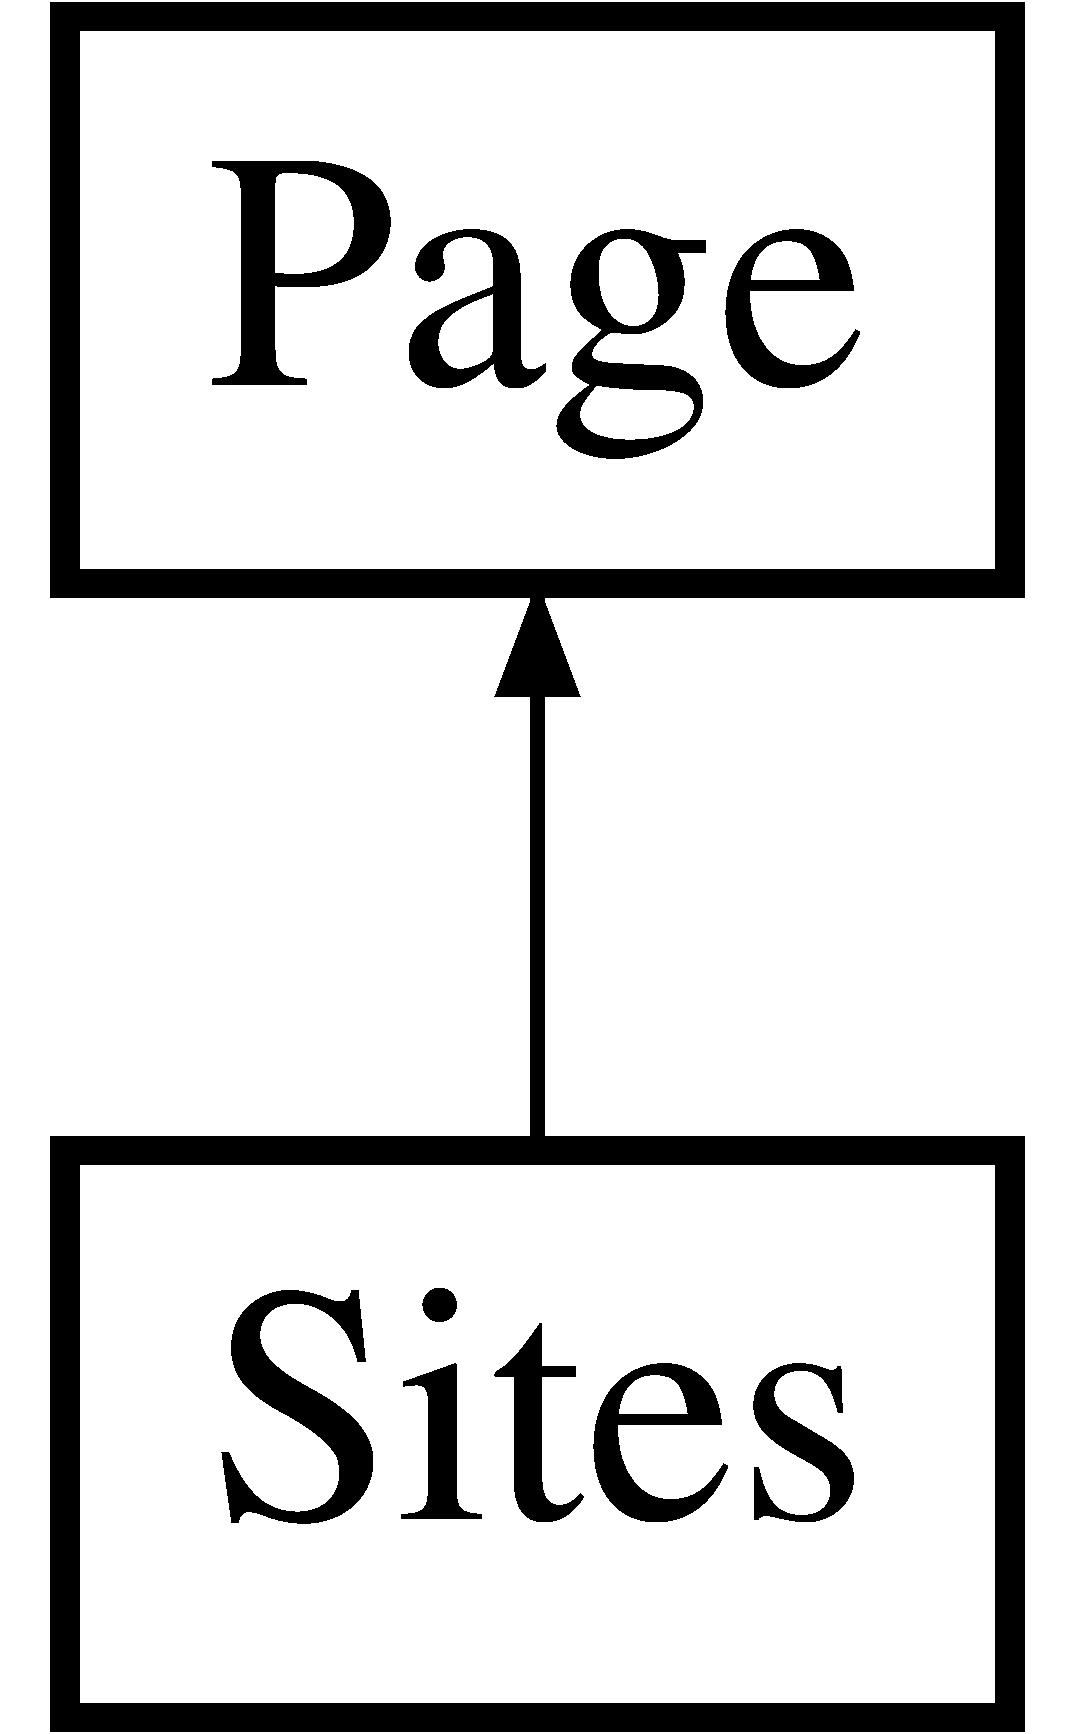
\includegraphics[height=2.000000cm]{class_sites}
\end{center}
\end{figure}
\subsection*{Protected Member Functions}
\begin{DoxyCompactItemize}
\item 
\hypertarget{class_sites_a3813c5de6d1f0499083db605115d464c}{void {\bfseries Page\+\_\+\+Load} (object sender, Event\+Args e)}\label{class_sites_a3813c5de6d1f0499083db605115d464c}

\end{DoxyCompactItemize}


The documentation for this class was generated from the following file\+:\begin{DoxyCompactItemize}
\item 
H\+D3web/Sites.\+aspx.\+cs\end{DoxyCompactItemize}

\hypertarget{class_tests}{\section{Tests Class Reference}
\label{class_tests}\index{Tests@{Tests}}
}
Inheritance diagram for Tests\+:\begin{figure}[H]
\begin{center}
\leavevmode
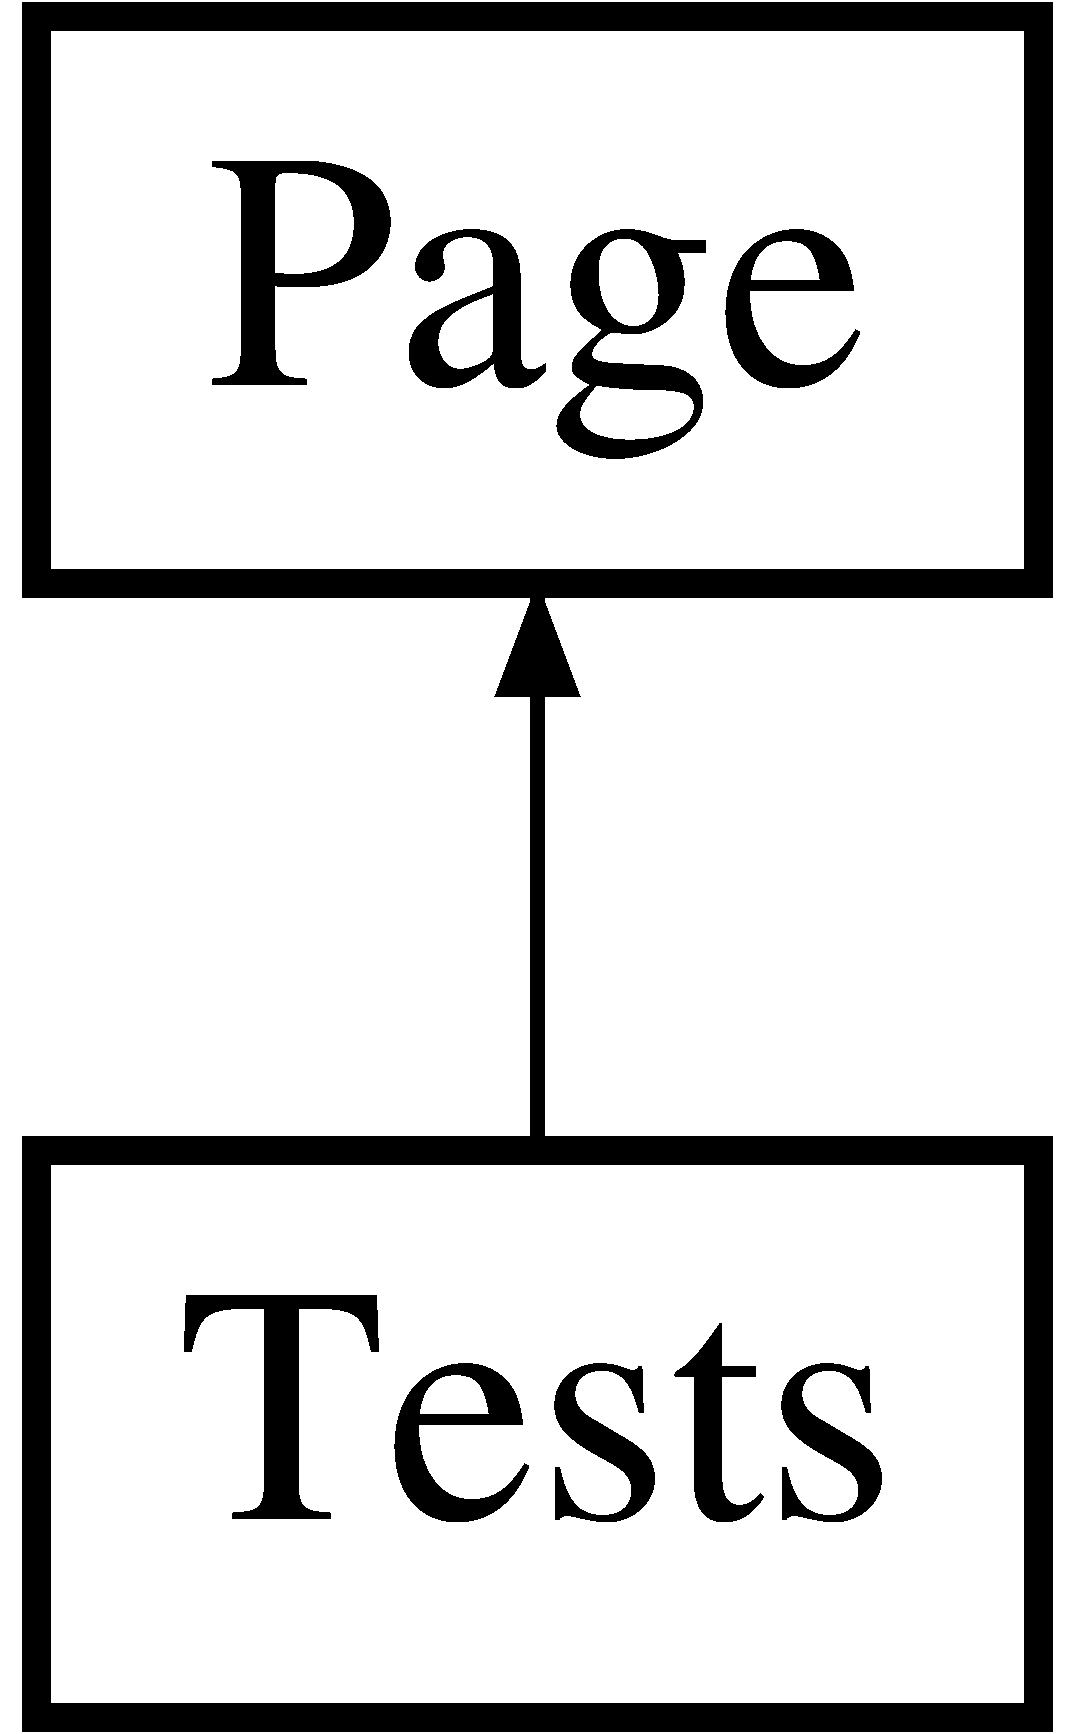
\includegraphics[height=2.000000cm]{class_tests}
\end{center}
\end{figure}
\subsection*{Protected Member Functions}
\begin{DoxyCompactItemize}
\item 
\hypertarget{class_tests_a98f2bec73f2c156815e27033d766b84d}{void {\bfseries Page\+\_\+\+Load} (object sender, Event\+Args e)}\label{class_tests_a98f2bec73f2c156815e27033d766b84d}

\end{DoxyCompactItemize}


The documentation for this class was generated from the following file\+:\begin{DoxyCompactItemize}
\item 
H\+D3web/Tests.\+aspx.\+cs\end{DoxyCompactItemize}

%--- End generated contents ---

% Index
\newpage
\phantomsection
\addcontentsline{toc}{chapter}{Index}
\printindex

\end{document}
